\documentclass[thesis]{thesis-gwu}[2018/08/31]

\usepackage{xspace}
\usepackage{xcolor} %remove if not needed at the end
\usepackage{multirow} 
\usepackage[utf8]{inputenc} % allows using accents directly in text, like ÔøΩ

\newcommand{\pygbe}{\texttt{PyGBe}\xspace}
\newcommand{\gmres}{\textsc{gmres}\xspace}
\newcommand{\bem}{\textsc{bem}\xspace}
\newcommand{\gpu}{\textsc{gpu}}
\newcommand{\cpu}{\textsc{cpu}}
\newcommand{\nvidia}{\textsc{nvidia}\xspace}
\newcommand{\msms}{\texttt{\textsc{msms}}\xspace}
\newcommand{\amber}{\texttt{\textsc{amber}}\xspace}
\newcommand{\ccby}{\textsc{cc-by}\xspace}
\newcommand{\bigO}{\mathcal{O}}
\renewcommand{\O}[1]{\mathcal{O}(#1)}
% !TEX root = ../thesis-sample.tex

% --------- FRONT MATTER PAGES ---------------------
% Title of the thesis
\title{COMPUTATIONAL NANOPLASMONICS FOR BIOSENSING APPLICATIONS: A BOUNDARY INTEGRAL IMPLEMENTATION IN THE QUASISTATIC LIMIT.}

% Author name
\author{Natalia Carolina Clementi}

% Previous degrees
\bsdepartment{Physics}
\bsschool{Universidad Nacional de C{\'o}rdoba.}
\bsgrad{2013}

\msdepartment{MS department}
\msschool{University}
\msgrad{year}
%\showmsdegree % you can show or hide the MS degree line 
\hidemsdegree

% PhD degree commands
% Committee
\showcommitteepage % hide this page if you're doing a MS thesis
%\hidecommitteepage 
\committee{ %
Lorena A. Barba, Professor of Mechanical and Aerospace Engineering,\\ 
Dissertation Director\\ % remember to add a space between committee members

Sanyia LeBlanc, Associate Professor of Mechanical and Aerospace Engineering,
Committee Member\\

Kausik Sarkar, Professor of Mechanical and Aerospace Engineering, \\
Committee Member\\

Yongsheng Leng, Professor of Mechanical and Aerospace Engineering, \\
Committee Member\\

Christopher Cooper Villagr{\'a}n, Assistant Professor of Mechanical Engineering,
Committee Member\\

}

% Chair must be entered separately for formatting reasons.
\chair{Lorena A. Barba}
\chairtitle{Professor of Mechanical and Aerospace Engineering}
% Department
\department{Mechanical and Aerospace Engineering}

\phdgrad{May 16, 2021}
\defensedate{February 19, 2021}
% Year of completion for copyright page and perhaps other places
\year=2021

% Copyright page
%\copyrightholder{Someone else}

% Dedication
\dedication{To all the women scientist to come. %
}

% Acknowledgments
\acknowledgments{
PENDING
}

% -----------------------------------------------------------------
% Typically only one of Preface/Foreward/Prologue would be in your thesis.
% To choose one simply delete the others and they will automatically dissappear

% Preface
\preface{
    This is the preface. 
    It's another front matter page that offers additional detail into your work.
    Typically, only one (preface OR prologue OR foreword) is used. 
    You can remove the other sections by deleting them inside \texttt{tex/frontmatter.tex} or using the appropriate show or hide commands.
}

\prologue{
    This is the prologe. 
    It's another front matter page that offers additional detail into your work.
    Typically, only one (preface OR prologue OR foreword) is used. 
    You can remove the other sections by deleting them inside \texttt{tex/frontmatter.tex} or using the appropriate show or hide commands.
}

\foreword[2]{
    This is the forword. 
    It's another front matter page that offers additional detail into your work.
    Typically, only one (preface OR prologue OR foreword) is used. 
    You can remove the other sections by deleting them inside \texttt{tex/frontmatter.tex} or using the appropriate show or hide commands.
}
% ----------------------------------------------------------------------

% commands to show or hide front matter pages

\showcopyright
\showabstract
\showcommitteepage
\showdedication
\showacknowledgments
\hidepreface
\hideprologue
\hideforeword

% ------------ TABLE OF CONTENTS ----------------------
% Commands to hide or show lists of figures, tables, etc.
\showlistoffigures
\showlistoftables
\hidenomenclature

\makeglossaries

% Some abstract text
\abstract{
This is the abstract. 
It contains some random text from 
}

%avoid indentation of paragraphs
\setlength\parindent{0pt}

%% DOCUMENT AREA
\begin{document}

% !TEX root = ../thesis-sample.tex

\chapter{Methods} \label{chap:methods}
\graphicspath{{methods/figs/}}

The first implementation of \pygbe relies on continuum electrostatics to compute the solvation energy
of biomolecules. This biomolecules are modeled as dielectric cavities inside an infinite continuum 
solvent, leading to a Poisson equation inside the molecules and Laplace or Poisson-Boltzmann
(accountability  of salt ions) in the solvent. The partial differential equations that model this problem
can be be expressed as boundary integral equations along the molecular interface, and solved using 
\pygbe's boundary element method implementation \cite{CooperBardhanBarba2013,CooperClementiBarba2015}.

% The original implementation of \pygbe used continuum electrostatic theory to compute
% the solvation energy of biomolecular systems. In that setting, biomolecules are modeled as 
% dielectric cavities inside an infinite continuum solvent, 
% leading to a Poisson equation inside the molecules and Laplace or Poisson-Boltzmann in the solvent medium (with appropriate boundary conditions).
% This set of partial differential equations can be 
% expressed with the corresponding boundary integral equation along the molecular interface.
% which \pygbe solves using a boundary element method \cite{CooperBardhanBarba2013,CooperClementiBarba2015}.

The present work extends \pygbe to the LSPR biosensing application. 
In the long-wavelength limit, Maxwell's equations can be approximated by a Laplace equation,
which permits using the methods implemented in \pygbe, with modifications
to allow for complex-valued permittivities, and to include the
effect of an external electric field.
This section describes the mathematical formulation for computing electromagnetic scattering 
in the long-wavelength setting, and develops the associated boundary integral equations 
and their discretized form.

\section{Scattering of small particles} \label{sec:scattering_small}

Electromagnetic scattering is usually modeled with Maxwell's equations. When the wavelength of the incoming wave is much larger than the
scatterer, these can be reduced to a \emph{quasi-static} 
first-order approximation \cite{MayergoyzZhang2007}:

\begin{align} \label{eq:electrostatic_scatter_E}
\nabla \cdot \mathbf{E}_{1s} &= 0 \qquad \nabla \times \mathbf{E}_{1s} = 0, \nonumber \\
\nabla \cdot \mathbf{E}_{2s} &= 0 \qquad \nabla \times \mathbf{E}_{2s} = 0, \nonumber \quad
\text{with interface conditions, } \nonumber \\
(\epsilon_1\mathbf{E}_{1s} &- \epsilon_2\mathbf{E}_{2s})\cdot\mathbf{n} = (\epsilon_2-\epsilon_1)\mathbf{E}_i\cdot \mathbf{n}.
\end{align}

In Equation \eqref{eq:electrostatic_scatter_E}, $\mathbf{E}_{1s}$ and $\mathbf{E}_{2s}$ 
are the electric fields of the scattered wave in the nanoparticle and host regions, respectively 
(see Figure \ref{fig:part_wave}), 
$\mathbf{E}_{i}$ is the field of the incoming wave, and $\epsilon_1$ 
and $\epsilon_2$ are the permittivities.
This approximation decouples the electric and magnetic fields, neglects the magnetic field, 
and describes the electric field as a curl-free vector field.
Hence, we can reformulate Equation \eqref{eq:electrostatic_scatter_E} with a scalar potential
($-\nabla \phi_{js} = \mathbf{E}_{js}$), as follows:
%
\begin{align} \label{eq:electrostatic_scatter}
\nabla^2 \phi_{1s} &= 0 \qquad \nabla^2 \phi_{2s} = 0 \qquad\text{on $\Omega_1$, $\Omega_2$} \nonumber \\
\epsilon_1\frac{\partial\phi_{1s}}{\partial \mathbf{n}} - \epsilon_2\frac{\partial\phi_{2s}}{\partial\mathbf{n}} &= (\epsilon_2-\epsilon_1)\frac{\partial\phi_i}{\partial\mathbf{n}} \quad \phi_{1s} = \phi_{2s} \quad \text{on $\Gamma$}.
\end{align}
%
Equation \eqref{eq:electrostatic_scatter} is an electrostatic equation 
with an imposed electric field $\mathbf{E}_i=-\nabla\phi_i$, where $\Gamma$ 
is the boundary between regions $\Omega_1$ and $\Omega_2$.

\begin{figure}%[h] %  figure placement: here, top, bottom, or page
   \centering
   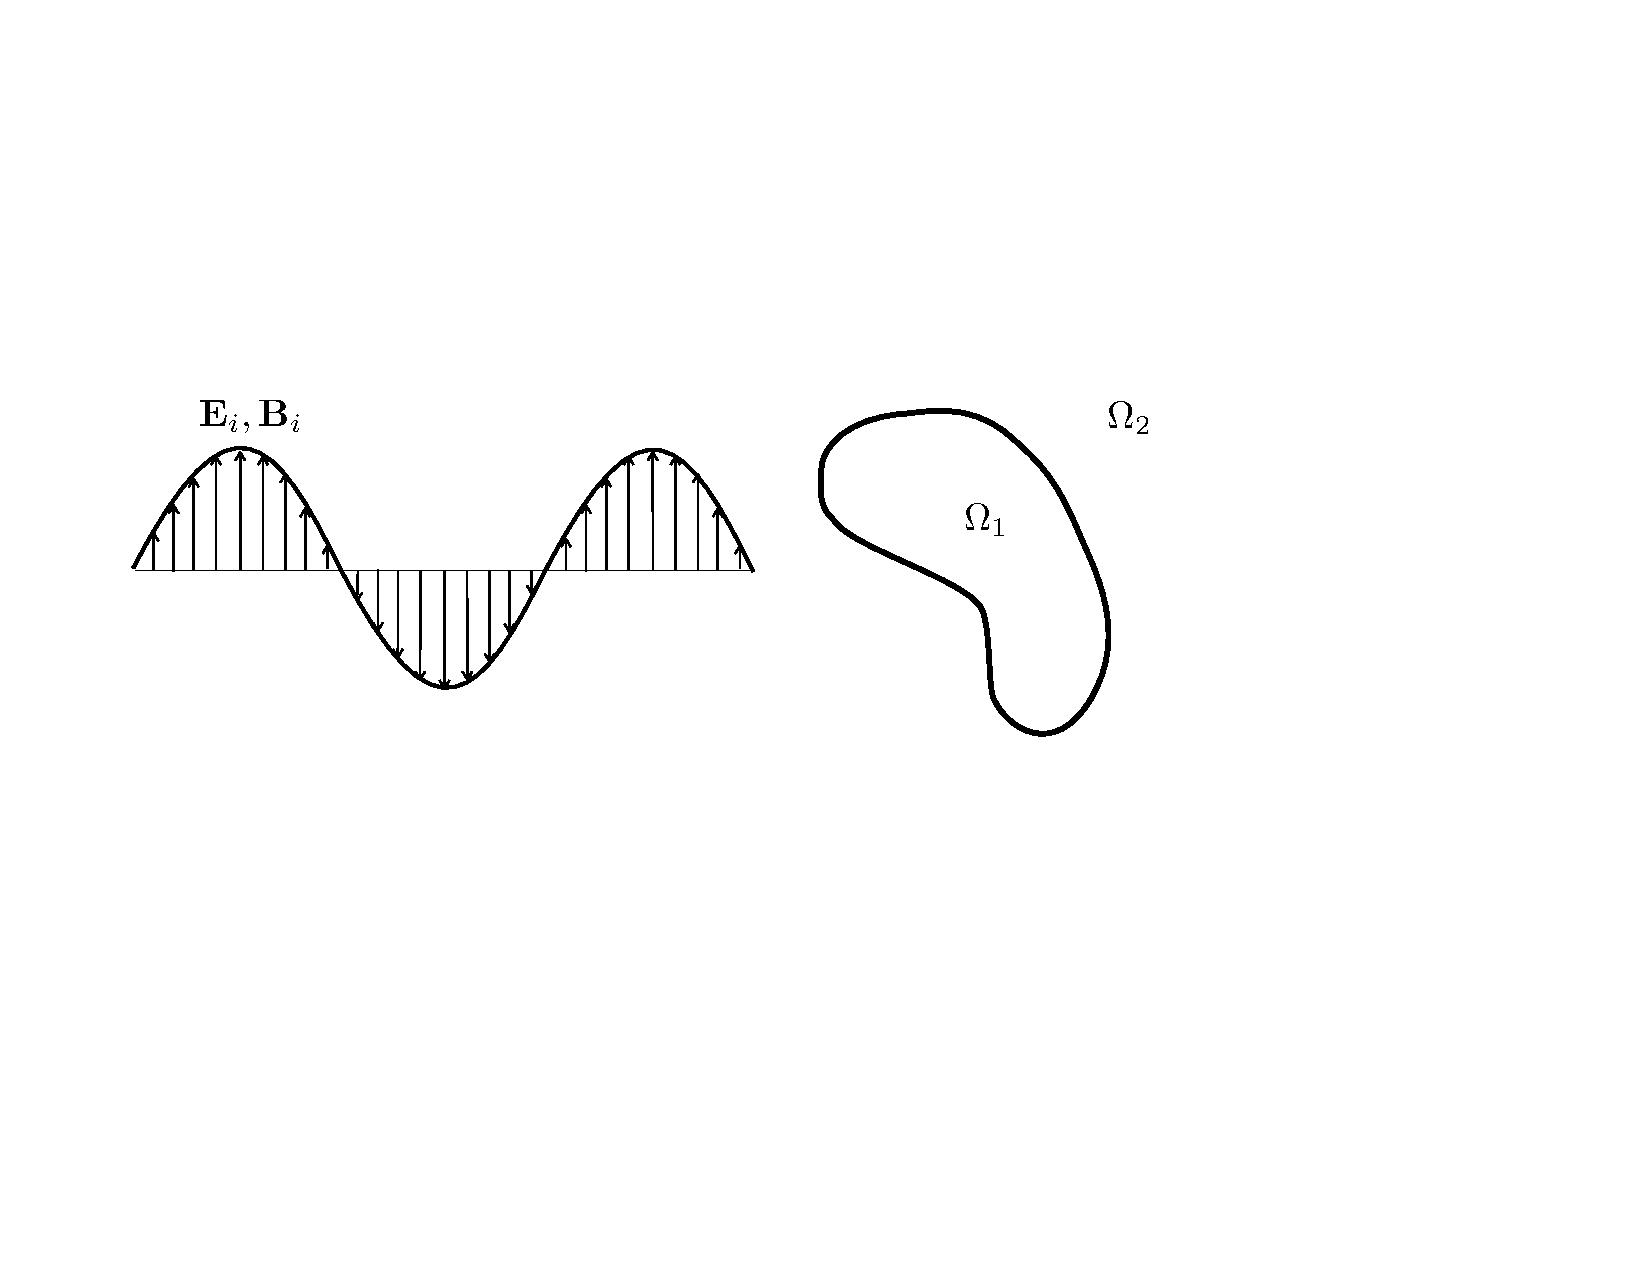
\includegraphics[width=0.55\textwidth]{particle_wave.pdf} 
   \caption{Nanoparticle interacting with an electromagnetic wave.}
   \label{fig:part_wave}
\end{figure}

\subsection{Far-field scattering} \label{sec:ff_scattering}

In LSPR, the scattered electromagnetic wave is measured by a detector located far away 
from the scatterer (nanoparticle), and plasmon resonance is identified when the energy 
detected is minimum. In the far-field limit, the scattered field
in the outside region ($\Omega_2$) is given by: 

\begin{equation} \label{eq:scat_efield_long_range}
    \mathbf{E}_{2s} = \frac{1}{4\pi\epsilon_2}k^2\frac{e^{ikr}}{r} (\mathbf{\hat{r}} \times \mathbf{p})\times\mathbf{\hat{r}}.
\end{equation} 

where $k=2\pi/\lambda$ is the wave number and $\lambda$ the wavelength, $\mathbf{\hat{r}}$ 
is a unit vector in the direction of the observation point, and $\mathbf{p}$ is
the dipole moment.
We can obtain the scattered field using the 
scattering amplitude \cite{Jackson}:

\begin{equation} \label{eq:scat_efield_fwa}
    \mathbf{E}_{2s}(\mathbf{r})_{r\to\infty} = \frac{e^{ikr}}{r} \mathbf{F}(\mathbf{k},\mathbf{k}_0),
\end{equation}

where $\mathbf{F}$ is the scattering amplitude, $\mathbf{k}$ is the 
scattered wave vector in the direction of propagation, and $\mathbf{k}_0$ the 
wave vector of the incident field. 

\subsection{Extinction cross-section and optical theorem} \label{sec:cext_ot}

The extinction cross-section ($C_\text{ext}$) is a measure of the energy that 
does not reach the detector, either because of scattering in other directions,
or absorption. This quantity is defined as the ratio between the lost energy and 
the intensity of the incoming wave, and has units of area. 
The extinction cross-section peaks at resonance of plasmons.

The extinction cross-section is related to the forward-scattering amplitude via the optical theorem. 
The traditional expression for this relationship applies for non-absorbing media 
\cite{MayergoyzZhang2007, Jackson}; 
Mishchenko \cite{Mishchenko2007} corrected it for absorbing media, 
giving an expression that can be re-written using Jackson's notation \cite{Jackson} as follows:

\begin{equation} \label{eq:cext_fwa}
    C_\text{ext} = \frac{4\pi}{k^\prime} \operatorname{Im} \left[ \frac{\mathbf{\hat{e}}_i}{|\mathbf{E}_i|}\mathbf{F}(\mathbf{k}=\mathbf{k}_0, \mathbf{k}_0) \right].
\end{equation}

Here, $k^\prime$ is the real part of the complex wave number, 

\begin{equation}
    k = k^\prime + ik^{\prime\prime} = \frac{2\pi}{\lambda} n,
\end{equation}

and $n$ is the refraction index of the host medium.

Combining Equations \eqref{eq:scat_efield_long_range} and \eqref{eq:scat_efield_fwa},
we can compute the scattering amplitude to then obtain the extinction cross-section 
with Equation \eqref{eq:cext_fwa}.


\section{The boundary element method} \label{sec:lspr_bem}

\subsection{Electrostatic potential of a nanoparticle under an electric field} \label{sec:pot_elec_field}

\subsubsection{Integral formulation}

The weak formulation of Laplace equation with test function $w$:

\begin{equation} \label{eq:lap_weak}
\int_\Omega \nabla^2 \phi(\mathbf{r}_\Omega') w(\mathbf{r}_\Omega') \text{d} \Omega^\prime= 0.
\end{equation}

where the evaluation point is $\mathbf{r}_\Omega$ a location in the domain $\Omega$.

If we use the Laplace's free-space Green's function as the test function $w$ we
get:

\begin{equation} \label{eq:lap_weak2}
\int_\Omega \nabla^2 \phi(\mathbf{r}'_\Omega) G_L(\mathbf{r}_\Omega,\mathbf{r}'_\Omega) \text{d} \Omega^\prime= 0.
\end{equation}

Manipulating the integrand using the product rule and later the divergence 
theorem, we get:

\begin{equation} \label{eq:lap_bie_dom}
\phi(\mathbf{r}_\Omega) = \oint_\Gamma G_L(\mathbf{r}_\Omega,\mathbf{r}'_\Gamma)  \frac{\partial} {\partial \mathbf{n}} \phi(\mathbf{r}'_\Gamma)  \text{d} \Gamma^\prime - \oint_\Gamma \phi(\mathbf{r}'_\Gamma)  \frac{\partial}{\partial \mathbf{n}} G_L(\mathbf{r}_\Omega,\mathbf{r}'_\Gamma) \text{d} \Gamma^\prime
\end{equation}

where \eqref{eq:lap_bie_dom}, $\mathbf{r}$ can be anywhere in the domain $\Omega$, 
and $\mathbf{r}'$ runs only on the boundary $\Gamma$. This equation has a 
singularity when $\mathbf{r}=\mathbf{r}'$. To handle this problem, we perform the
integral on a surface $\Gamma'$ that is like $\Gamma$ but with a hemisphere of 
radius $\varepsilon$ center at $\mathbf{r}$. We split the integrals into the part
that we have no singularity and the part that has the hemisphere. After solving these
equations when $\varepsilon \to 0$, equation \eqref{eq:lap_bie_dom} results in:

\begin{equation} \label{eq:lap_bie}
\frac{\phi(\mathbf{r}_\Gamma)}{2} +  \oint_\Gamma \phi(\mathbf{r}'_\Gamma)  \frac{\partial}{\partial \mathbf{n}} G_L(\mathbf{r}_\Gamma,\mathbf{r}'_\Gamma) \text{d} \Gamma^\prime = \oint_\Gamma G_L(\mathbf{r}_\Gamma,\mathbf{r}'_\Gamma)  \frac{\partial} {\partial \mathbf{n}} \phi(\mathbf{r}'_\Gamma)  \text{d} \Gamma^\prime,
\end{equation}

where these are Cauchy principal value integrals.

Using the single and double layer operators:

\begin{equation}\label{eq:single_layer}
   V^{\Gamma}_L (\psi(\mathbf{r}_\Gamma)) = \oint_\Gamma \psi(\mathbf{r}'_\Gamma) G_L(\mathbf{r}_\Gamma, \mathbf{r}'_\Gamma) \text{d} \Gamma',
   \end{equation}
   %
   \begin{equation}\label{eq:double_layer}
   K^{\Gamma}_L (\psi(\mathbf{r}_\Gamma)) = \oint_\Gamma \psi(\mathbf{r}'_\Gamma) \frac{\partial}{\partial \mathbf{n}}G_L(\mathbf{r}_\Gamma, \mathbf{r}'_\Gamma) \text{d} \Gamma'.
   \end{equation}
   %
   Here, $G_L$ is the free-space Green's function of the Laplace equation:
   %
   \begin{equation}
   G_L(\mathbf{r},\mathbf{r}') = \frac{1}{4\pi|\mathbf{r}-\mathbf{r}'|}
   \end{equation}
   

We can rewrite equation \eqref{eq:lap_bie} using the operator notation, as:

\begin{equation} \label{eq:lap_operator}
\left[ \frac{\mathbb{I}}{2} + K_L^{\mathbf{r}_\Gamma} \right] \left( \phi_\Gamma \right) = V_L^{\mathbf{r}_\Gamma} \left( \frac{\partial}{\partial \mathbf{n}} \phi_\Gamma \right),
\end{equation}

where $\mathbb{I}$ is the identity operator.

Following the same steps we can write the system of partial differential equations 
in Equation \eqref{eq:electrostatic_scatter} as a system 
of boundary integral equations \cite{BrebbiaDominguez1992}. Evaluating on the surface $\Gamma$, this
becomes
%
\begin{align} \label{eq:integral_eq_lspr_nobc}
\frac{\phi_{1s,\Gamma}}{2}+ K_{L}^{\Gamma}(\phi_{1s,\Gamma}) - V_{L}^{\Gamma} \left(\frac{\partial}{\partial \mathbf{n}}\phi_{1s,\Gamma} \right) = 0&  \nonumber \\
\frac{\phi_{2s,\Gamma}}{2} - K_{L}^{\Gamma}(\phi_{2s,\Gamma}) + V_{L}^{\Gamma} \left( \frac{\partial}{\partial \mathbf{n}} \phi_{2s,\Gamma} \right) = 0&,
\end{align}
%
where $V$ and $K$ are the single- and double-layer operators.
%
Applying the interface conditions of Equation \eqref{eq:electrostatic_scatter},
leads to:

\begin{align} \label{eq:integral_eq_lspr}
\frac{\phi_{1s,\Gamma}}{2}+ K_{L}^{\Gamma}(\phi_{1s,\Gamma}) - V_{L}^{\Gamma} \left(\frac{\partial}{\partial \mathbf{n}}\phi_{1s,\Gamma} \right) &= 0  \nonumber \\
\frac{\phi_{1s,\Gamma}}{2} - K_{L}^{\Gamma}(\phi_{1s,\Gamma}) + \frac{\epsilon_1}{\epsilon_2}V_{L}^{\Gamma} \left( \frac{\partial}{\partial \mathbf{n}} \phi_{1s,\Gamma}  \right) &=
 \frac{\epsilon_2-\epsilon_1}{\epsilon_2}V_{L}^{\Gamma}\left( \frac{\partial}{\partial \mathbf{n}} \phi_{i,\Gamma} \right)\quad \text{on $\Gamma$.}
\end{align}



\subsection{Analyte-sensor electrostatic potential under an electric field}

The sketch in Figure \ref{fig:analyte-sensor} shows a metallic nanoparticle ($\Omega_1$) interacting with an analyte ($\Omega_3$), under an external electric field.
Mathematically, this situation can be modeled as

\begin{align}\label{eq:electrostatic_scatter_prot_sen}
\nabla^2 \phi_{1s} &= 0, \qquad \nabla^2 \phi_{2s} = 0 \qquad\text{on $\Omega_1$, $\Omega_2$} \nonumber\\
\nabla^2 \phi_{3s} &= -\frac{1}{\epsilon_3} \sum_{k=0}^{N_q} \delta(|\mathbf{r}-\mathbf{r}_k|) q_k \qquad\text{on $\Omega_3$} \nonumber \\
\epsilon_1\frac{\partial\phi_{1s}}{\partial \mathbf{n}} - \epsilon_2\frac{\partial\phi_{2s}}{\partial\mathbf{n}} &= (\epsilon_2-\epsilon_1)\frac{\partial\phi_i}{\partial\mathbf{n}} \quad \phi_{1s} = \phi_{2s} \quad \text{on $\Gamma_1$}. \nonumber\\
\epsilon_3\frac{\partial\phi_{3s}}{\partial \mathbf{n}} - \epsilon_2\frac{\partial\phi_{2s}}{\partial\mathbf{n}} &= (\epsilon_2-\epsilon_3)\frac{\partial\phi_i}{\partial\mathbf{n}} \quad \phi_{3s} = \phi_{2s} \quad \text{on $\Gamma_2$}.
\end{align}
%
where $q_k$ are the point charges of the atoms inside the protein, located at $\mathbf{r}_k$.

\subsubsection{Integral formulation}

Similar to Equation \eqref{eq:integral_eq_lspr}, we can write the system of partial differential equations in \eqref{eq:electrostatic_scatter_prot_sen} as

\begin{align} \label{eq:integral_eq_lspr_nobc_system}
\frac{\phi_{1s,\Gamma_1}}{2}+ K_{L,\Gamma_1}^{\Gamma_1}(\phi_{1s,\Gamma_1}) &- V_{L,\Gamma_1}^{\Gamma_1} \left(\frac{\partial}{\partial \mathbf{n}}\phi_{1s,\Gamma_1} \right) = 0  \nonumber \\
\frac{\phi_{2s,\Gamma_1}}{2} - K_{L,\Gamma_1}^{\Gamma_1}(\phi_{2s,\Gamma_1}) + V_{L,\Gamma_1}^{\Gamma_1} \left(\frac{\partial}{\partial \mathbf{n}}\phi_{2s,\Gamma_1} \right) 
& - K_{L,\Gamma_2}^{\Gamma_1}(\phi_{2s,\Gamma_2}) + V_{L,\Gamma_2}^{\Gamma_1} \left(\frac{\partial}{\partial \mathbf{n}}\phi_{2s,\Gamma_2} \right) = 0  \nonumber \\
\frac{\phi_{2s,\Gamma_2}}{2} - K_{L,\Gamma_1}^{\Gamma_2}(\phi_{2s,\Gamma_1}) + V_{L,\Gamma_1}^{\Gamma_2} \left(\frac{\partial}{\partial \mathbf{n}}\phi_{2s,\Gamma_1} \right)  
&- K_{L,\Gamma_2}^{\Gamma_2}(\phi_{2s,\Gamma_2}) + V_{L,\Gamma_2}^{\Gamma_2} \left(\frac{\partial}{\partial \mathbf{n}}\phi_{2s,\Gamma_2} \right) = 0  \nonumber \\
\frac{\phi_{3s,\Gamma_2}}{2} + K_{L,\Gamma_2}^{\Gamma_2}(\phi_{3s,\Gamma_2}) &- V_{L,\Gamma_2}^{\Gamma_2} \left( \frac{\partial}{\partial \mathbf{n}} \phi_{3s,\Gamma_2} \right) = \frac{1}{4\pi\epsilon_3} \sum_{k=0}^{N_q} \frac{q_k}{|\mathbf{r}_{\Gamma_2} - \mathbf{r}_k|} ,
\end{align}
%
where $V$ and $K$ are the single- and double-layer operators in equations 
\eqref{eq:single_layer} and \eqref{eq:double_layer}. In this case, we distinguish between the
surface where the integrals run (subindex), and the surface that contains the evaluation point (superindex).

Applying the interface conditions of equation \eqref{eq:electrostatic_scatter_prot_sen},
leads to: 

\begin{align} \label{eq:integral_eq_lspr_system}
\frac{\phi_{1s,\Gamma_1}}{2}&+ K_{L,\Gamma_1}^{\Gamma_1}(\phi_{1s,\Gamma_1}) - V_{L,\Gamma_1}^{\Gamma_1} \left(\frac{\partial}{\partial \mathbf{n}}\phi_{1s,\Gamma_1} \right) = 0  \nonumber \\
 \frac{\phi_{1s,\Gamma_1}}{2}& - K_{L,\Gamma_1}^{\Gamma_1}(\phi_{1s,\Gamma_1}) + V_{L,\Gamma_1}^{\Gamma_1} \left(\frac{\epsilon_1}{\epsilon_2}\frac{\partial}{\partial \mathbf{n}}\phi_{1s,\Gamma_1} \right) - V_{L,\Gamma_1}^{\Gamma_1} \left(\frac{\epsilon_2-\epsilon_1}{\epsilon_2}\frac{\partial}{\partial \mathbf{n}}\phi_{i,\Gamma_1} \right) \nonumber\\ 
 & - K_{L,\Gamma_2}^{\Gamma_1}(\phi_{3s,\Gamma_2}) + V_{L,\Gamma_2}^{\Gamma_1} \left(\frac{\epsilon_3}{\epsilon_2}\frac{\partial}{\partial \mathbf{n}}\phi_{3s,\Gamma_2} \right)  - V_{L,\Gamma_2}^{\Gamma_1} \left(\frac{\epsilon_2 -\epsilon_3}{\epsilon_2}\frac{\partial}{\partial \mathbf{n}}\phi_{i,\Gamma_2} \right) = 0   \nonumber \\
 \frac{\phi_{3s,\Gamma_1}}{2}& - K_{L,\Gamma_1}^{\Gamma_2}(\phi_{1s,\Gamma_1}) + V_{L,\Gamma_1}^{\Gamma_2} \left(\frac{\epsilon_1}{\epsilon_2}\frac{\partial}{\partial \mathbf{n}}\phi_{1s,\Gamma_1} \right) - V_{L,\Gamma_1}^{\Gamma_2} \left(\frac{\epsilon_2-\epsilon_1}{\epsilon_2}\frac{\partial}{\partial \mathbf{n}}\phi_{i,\Gamma_1} \right) \nonumber \\
& - K_{L,\Gamma_2}^{\Gamma_2}(\phi_{3s,\Gamma_2}) + V_{L,\Gamma_2}^{\Gamma_2} \left(\frac{\epsilon_3}{\epsilon_2}\frac{\partial}{\partial \mathbf{n}}\phi_{3s,\Gamma_2} \right)  - V_{L,\Gamma_2}^{\Gamma_2} \left(\frac{\epsilon_2 -\epsilon_3}{\epsilon_2}\frac{\partial}{\partial \mathbf{n}}\phi_{i,\Gamma_2} \right) = 0  \nonumber \\
\frac{\phi_{3s,\Gamma_2}}{2}& + K_{L,\Gamma_2}^{\Gamma_2}(\phi_{3s,\Gamma_2}) - V_{L,\Gamma_2}^{\Gamma_2} \left( \frac{\partial}{\partial \mathbf{n}} \phi_{3s,\Gamma_2} \right) = \frac{1}{4\pi\epsilon_3} \sum_{k=0}^{N_q} \frac{q_k}{|\mathbf{r}_{\Gamma_2} - \mathbf{r}_k|} 
\end{align}

\begin{figure}%[b] %  figure placement: here, top, bottom, or page
    \centering
    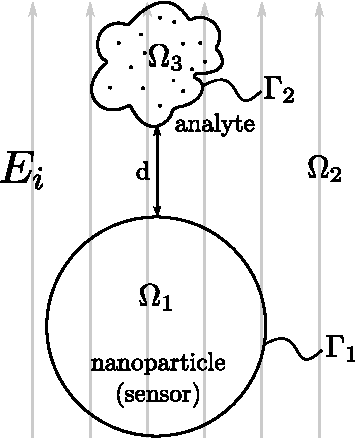
\includegraphics[width=0.35\textwidth]{protein_sensor_regions.pdf} 
    \caption{Analyte-sensor system under electric field.}
    \label{fig:analyte-sensor}
 \end{figure}

\paragraph{Discretization and linear system}

We discretize the surface into flat triangles, and assume that  $\phi$ and 
$\partial \phi/\partial \mathbf{n}$ are constant within each element. We can
then write the layer operators in their discretized form as follows:
%
\begin{align} \label{eq:layers_disc}
V_{L,\text{disc}}^{\mathbf{r}_\Gamma} \left( \frac{\partial}{\partial \mathbf{n}} \phi(\mathbf{r}_{\Gamma}) \right) &= \sum_{j=1}^{N_p} \frac{\partial}{\partial \mathbf{n}} \phi(\mathbf{r}_{\Gamma_j}) \int_{\Gamma_j} G_L(\mathbf{r}_\Gamma,\mathbf{r}_{\Gamma_j})  \mathrm{d} \Gamma_j  \nonumber \\
K_{L,\text{disc}}^{\mathbf{r}_\Gamma}(\phi(\mathbf{r}_{\Gamma})) &=  \sum_{j=1}^{N_p}\phi(\mathbf{r}_{\Gamma_j})\int_{\Gamma_j} \frac{\partial}{\partial \mathbf{n}} \left[ G_L(\mathbf{r}_\Gamma,\mathbf{r}_{\Gamma_j}) \right]\mathrm{d} \Gamma_j
\end{align}
%
where $N_p$ is the number of discretization elements on $\Gamma$, 
and $\phi(\mathbf{r}_{\Gamma_j})$ and $\frac{\partial}{\partial \mathbf{n}} 
\phi(\mathbf{r}_{\Gamma_j})$ are the values of $\phi$ and 
$\frac{\partial \phi}{\partial \mathbf{n}}$ on panel $\Gamma_j$.
Using centroid collocation, we can write equation \eqref{eq:integral_eq_lspr} in matrix form as:
%
 \begin{equation} \label{eq:matrix_lspr}
 \left[
    \begin{matrix} 
       \frac{1}{2} + K_{L}^{\Gamma} & -V_{L}^{\Gamma}  \vspace{0.2cm} \\
       \frac{1}{2} - K_{L}^{\Gamma} &  \frac{\epsilon_1}{\epsilon_2} V_{L}^{\Gamma}  \vspace{0.2cm} 
    \end{matrix}
    \right] \left[ 
    \begin{matrix} 
       \phi_{1s,\Gamma} \vspace{0.2cm} \\
       \frac{\partial}{\partial \mathbf{n}} \phi_{1s,\Gamma} \vspace{0.2cm}
    \end{matrix} 
     \right] =   
    \left[
    \begin{matrix} 
       0 \\
       V_{L}^{\Gamma} \left(\frac{\epsilon_2-\epsilon_1}{\epsilon_2}\right) \frac{\partial\phi_i}{\partial\mathbf{n}} \vspace{0.2cm} 
    \end{matrix}
    \right]
 \end{equation}
%
Equation \eqref{eq:integral_eq_lspr_system} can be represented as:
%
\begin{align} \label{eq:matrix_multi}
 \left[
    \begin{matrix} 
       \frac{1}{2}+K_{L, \Gamma_1}^{\Gamma_1} & -V_{L, \Gamma_1}^{\Gamma_1} & 0 &  0   \vspace{0.2cm} \\
       \frac{1}{2}-K_{L, \Gamma_1}^{\Gamma_1} & \frac{\epsilon_1}{\epsilon_2} V_{L, \Gamma_1}^{\Gamma_1} & -K_{L, \Gamma_2}^{\Gamma_1} & \frac{\epsilon_3}{\epsilon_2} V_{L, \Gamma_2}^{\Gamma_1} \vspace{0.2cm}  \\
        -K_{L, \Gamma_1}^{\Gamma_2}&\frac{\epsilon_1}{\epsilon_2} V_{L, \Gamma_1}^{\Gamma_2} & \frac{1}{2}-K_{L, \Gamma_2}^{\Gamma_2}  &  \frac{\epsilon_3}{\epsilon_2} V_{L, \Gamma_2}^{\Gamma_2} \vspace{0.2cm} \\
       0 & 0 & \frac{1}{2}+K_{L, \Gamma_2}^{\Gamma_2}&  - V_{L, \Gamma_2}^{\Gamma_2}   \vspace{0.2cm} \\
    \end{matrix}
    \right] 
\cdot
 \left[
    \begin{matrix}
    \phi_{1,\Gamma_1} \vspace{0.2cm} \\
    \frac{\partial}{\partial \mathbf{n}} \phi_{1,\Gamma_1} \vspace{0.2cm} \\
    \phi_{3,\Gamma_2} \vspace{0.2cm} \\
    \frac{\partial}{\partial \mathbf{n}} \phi_{3,\Gamma_2} \vspace{0.2cm} \\
    \end{matrix}
\right]&
 \nonumber \\
 = \left[
    \begin{matrix}
    0 \vspace{0.2cm} \\
    V_{L,\Gamma_1}^{\Gamma_1} \left(\frac{\epsilon_2-\epsilon_1}{\epsilon_2}\frac{\partial}{\partial \mathbf{n}}\phi_{i,\Gamma_1} \right)
    + V_{L,\Gamma_2}^{\Gamma_1} \left(\frac{\epsilon_2 -\epsilon_3}{\epsilon_2}\frac{\partial}{\partial \mathbf{n}}\phi_{i,\Gamma_2} \right)
    \vspace{0.2cm}\\
    V_{L,\Gamma_1}^{\Gamma_2} \left(\frac{\epsilon_2-\epsilon_1}{\epsilon_2}\frac{\partial}{\partial \mathbf{n}}\phi_{i,\Gamma_1} \right)
    + V_{L,\Gamma_2}^{\Gamma_2} \left(\frac{\epsilon_2 -\epsilon_3}{\epsilon_2}\frac{\partial}{\partial \mathbf{n}}\phi_{i,\Gamma_2} \right)
    \vspace{0.2cm}\\
    \frac{1}{4\pi\epsilon_3}\sum_{k=0}^{N_q} \frac{q_k}{|\mathbf{r}_{\Gamma_2} - \mathbf{r}_k|} \vspace{0.2cm}  \\
    \end{matrix}
\right]&
\end{align}
%
where the elements of the matrix are
% %
\begin{align} \label{eq:layers_element}
V_{L,ij}^{\Gamma} &= \int_{\Gamma_j} G_L(\mathbf{r}_{\Gamma_i},\mathbf{r}_{\Gamma_j})  \mathrm{d} \Gamma_j, \nonumber \\
K_{L,ij}^{\Gamma} &= \int_{\Gamma_j} \frac{\partial}{\partial \mathbf{n}} \left[ G_L(\mathbf{r}_{\Gamma_i},\mathbf{r}_{\Gamma_j}) \right]\mathrm{d} \Gamma_j,
\end{align}
%
with $\mathbf{r}_{\Gamma_i}$ being at the center of panel $\Gamma_i$.


\paragraph{Integral evaluation}

We evaluate the integrals in Equation \eqref{eq:layers_element} with Gauss quadrature
rules. The $1/r$ singularity of the Green's function poses a
problem to obtaining good accuracy when the integral is 
singular or near-singular. Therefore, we define three different regions, as follows.
\begin{description}

\item[Singular integrals:] If the collocation point is in the integration element,
the singularity is difficult to resolve with standard
Gauss integration schemes. In this case, we use a semi-analytical technique 
\cite{HessSmith1967,ZhuHuangSongWhite2001} that places $N_k$ quadrature nodes on the 
edges of the triangle.

\item[Near-singular integrals:] If the collocation point is close to the integration element,
the integrand has a high gradient, and high-order quadrature rules are required. 
We use the representative length of the integrated triangle ($L = \sqrt{2\cdot\text{Area}}$)
to define a threshold of the \emph{nearby} region, for example, when the integration panel 
is $2L$ or less away from the collocation point. For near-singular integrals, we use 
$K_{fine}=19, 25  \text{ or }  37$ points per triangle. 

\item[Far-away integrals:] When the distance between the collocation point and the integration
element is beyond the threshold, they are considered to be far-away. 
At this point, the integrand is smooth enough that we obtain good 
accuracy with low-order integration, for example, with 
$K=1, 3  \text{ or } 4$ Gauss quadrature points per boundary element. 
\end{description}

\subsubsection{Boundary integral expression of the dipole moment}

As shown in Equation \eqref{eq:scat_efield_long_range}, the scattered electric 
field in the far-away limit depends on the dipole moment. The dipole moment is 
defined as 
%
\begin{equation} \label{eq:dipole_def}
\mathbf{p} = \int_\Omega \mathbf{r} \rho \text{d}\Omega,
\end{equation}
%
and rewriting this equation using Gauss' law, we obtain
%
\begin{equation} \label{eq:dipole_def_gauss}
\mathbf{p} = -\epsilon_2\int_\Omega \mathbf{r} \nabla^2 \phi_{2s} \text{d}\Omega.
\end{equation}
%
For component $i$, this becomes:
%
\begin{equation} \label{eq:dipole_def_gauss_i}
{p_i} = -\epsilon_2\int_\Omega {x_i} \nabla^2 \phi_{2s} \text{d}\Omega.
\end{equation}
%
Using the identity
%
\begin{equation} \label{eq:identity_grad}
  \nabla \cdot \left(f \mathbf{v}\right) = \left( \nabla f \right)\cdot \mathbf{v} + f\left(\nabla \cdot \mathbf{v}\right)
\end{equation}
%
with $f=x_i$ and $\mathbf{v} = \nabla\phi_{2s}$, we can rewrite Equation \eqref{eq:dipole_def_gauss_i}
as 
%
\begin{equation}
- \frac{p_i}{\epsilon_2} = \int_\Omega \nabla \cdot \left( x_i \nabla \phi_{2s} \right) \; \text{d}\Omega - \int_\Omega \nabla x_i \cdot \nabla\phi_{2s} \; \text{d}\Omega, \nonumber 
\end{equation}
 and applying the divergence theorem
\begin{equation} \label{eq:dip_gauss_interm_1}
- \frac{p_i}{\epsilon_2}= \oint_\Gamma  x_i  \nabla \phi_{2s} \cdot \mathbf{n} \; \text{d}\Gamma - \int_\Omega \nabla x_i \cdot \nabla\phi_{2s} \; \text{d}\Omega.
\end{equation}
%
Using the identity \eqref{eq:identity_grad} again in Equation \eqref{eq:dip_gauss_interm_1}, this time 
taking $f=\phi_{2s}$ and $\mathbf{v} = \nabla x_i$, we get:
%
\begin{align} \label{eq:dip_gauss_interm_2}
 - \frac{p_i}{\epsilon_2} =& \oint_\Gamma  x_i  \frac{\partial \phi_{2s}}{\partial \mathbf{n}} \text{d}\Gamma - \nonumber \\
 & \left[ \int_\Omega \nabla \cdot \left( \phi_{2s} \nabla x_i \right)\;\text{d}\Omega - \int_\Omega  \phi_{2s} \nabla^2 x_i \;\text{d}\Omega\right] \nonumber\\
%&\text{and applying the divergence theorem} \nonumber \\
=& \oint_\Gamma  x_i  \frac{\partial \phi_{2s}}{\partial \mathbf{n}} \; \text{d}\Gamma - \oint_\Gamma \phi_{2s} \nabla x_i \cdot \mathbf{n} \; \text{d}\Gamma \nonumber \\
=& \oint_\Gamma  x_i  \frac{\partial \phi_{2s}}{\partial \mathbf{n}} \; \text{d}\Gamma - \oint_\Gamma \phi_{2s} n_i \;\text{d}\Gamma
\end{align}
%
Throughout this derivation, the normals are pointing into $\Omega_1$. However, in our implementation 
all normals are pointing outwards, and we need to include an extra negative sign, yielding:
%
\begin{equation} \label{eq:dipole_def_gauss_i_final}
{p_i} = \epsilon_2 \left[ \oint_\Gamma  x_i  \frac{\partial \phi_{2s}}{\partial \mathbf{n}} \text{d}\Gamma - \oint_\Gamma \phi_{2s} n_i \; \text{d}\Gamma \right].
\end{equation}

Using BEM, we obtain the electrostatic potential and its normal derivative, on the surface of the nanoparticle, 
which we use in Equation \eqref{eq:dipole_def_gauss_i_final} to get the dipole 
moment, and in Equation \eqref{eq:scat_efield_long_range} to obtain the scattered
electric field. We can then use Equation \eqref{eq:scat_efield_fwa} and Equation 
\eqref{eq:cext_fwa} to get the extinction cross section.


\subsection{Acceleration strategies} \label{sec:acc_strategies}

One disadvantage of the Boundary Element Method (BEM) is that it generates dense matrices
after discretization. Solving the resulting linear system using
Gaussian elimination would require $\O{N^3}$ computations and $\O{N^2}$ storage, whereas for a
Krylov-subspace iterative solver, like the Generalized Minimal Residual Method (GMRES),
computations drop to $\O{N^2}$ because they are dominated by dense matrix-vector 
products. This makes BEM inefficient with more than a few thousand boundary elements,
which are the mesh sizes required for real applications. 

In our formulation with Gaussian quadrature and collocation, the matrix-vector product
becomes an $N$-body problem, with Gauss nodes acting as centers of mass (\emph{sources}), 
and the collocation points acting as evaluation points for the potential (\emph{targets}).
To overcome the unfavorable scaling,
we accelerate the matrix-vector product using a treecode algorithm \cite{BarnesHut1986,DuanKrasny2001}, 
which is a fast-summation algorithm capable of reducing $\O{N^2}$
computational patterns like

\begin{equation} \label{eq:summation}
V(\mathbf{x}_i) = \sum_{j=1}^{N} q_j \psi(\mathbf{x}_i, \mathbf{y}_j) 
\end{equation}
%
to a computational complexity of $\O{N \log N}$. In Equation \eqref{eq:summation} 
$q_j$ is the weight, $\psi$ the kernel, $\mathbf{y}_j$ the locations of sources and 
$\mathbf{x}_i$ the locations of targets.

The treecode groups sources geometrically in boxes of an octree, built ensuring
that no box in the lowest level has more than $N_\text{crit}$ sources. If a group of
sources is far away from a target, their influence is aggregated at an expansion center,
and the target interacts with the box, rather than with each source independently.
If the group of targets is  close, the treecode queries the child
boxes. If the box has no children and still is not far enough, the interaction is 
performed directly via \eqref{eq:summation}.
 The threshold to decide if a box is far enough is called the multipole-
acceptance criterion (MAC), defined as:
%
\begin{equation}
\theta > \frac{r_b}{r},
\end{equation}
%
where $r_b$ is the box size and $r$ the distance between the box center and the target.
Common values of $\theta$ are $1/2$ and $2/3$.
To approximate the contribution of the sources, we use Taylor expansions
of order $P$.
The treecode allows us to control the accuracy of the approximation by modifying $\theta$ and $P$.
Further details of the treecode implementation in \pygbe can be found in \cite{CooperBarba-share154331,CooperBardhanBarba2013}.

\subsection{Richardson extrapolation} \label{sec:rich_extrapolation}

In numerical computing, Richardson extrapolation is a technique used to get an estimation
of the exact solution from multiple computations using consecutive resolutions from coarser
to finer. In order to be applied, all the computations used need to converge to the exact value
at a constant rate, in other words, they are in the asymptotic range. When these conditions are met,
we can compute an estimate of the exact solution as:

\begin{equation} \label{eq:rich_extr}
   f_{\text{exact}} \approx f_1 + \frac{f_1 - f_2}{r^{p} - 1},
\end{equation} 

where $f_1$ and $f_2$ are the solutions at the fine and coarse grid, respectively, 
$r$ is the mesh refinement ratio, and $p$ is the order of convergence.

To use Equation \eqref{eq:rich_extr} we need to make sure that $f_1$ and $f_2$ are in the 
asymptotic regime. We compute the \textit{observed} order of convergence $p$ from three grid resolutions
refined at constant ratio $r$:

\begin{equation} \label{eq:observed_order}
   p = \frac{\log \left( \frac{f_3 - f_2}{f_2-f_1} \right)}{\log (r)}.
\end{equation}
   
and if the result of Eq. \eqref{eq:observed_order} matches the \textit{expected} order of convergence
of the method, this indicates that the computations for $f_1$, $f_2$ and $f_3$ are in the asymptotic range.
Once we know that our $f_i$'s are in the asymptotic range, we can use Eq. \eqref{eq:rich_extr} and replacing
the computed $p$ to get the estimated exact solution. We can also compute the estimated exact solution
directly from the values of $f_1$, $f_2$ and $f_3$ by doing some algebra on \eqref{eq:rich_extr}.

We know that $\log_r(x) = \log(x)/\log(r)$ and $r^{\log_r(x)} = x$. If we set $x = (f_3 - f_2)/(f_2 -f_1)$ 
then we can write Eq. \eqref{eq:observed_order}:

\begin{align} \label{eq:rich_extr2}
   f_{\text{exact}} &\approx f_1 + \frac{(f_1 - f_2)(f_2 -f_1)}{f_3-2f_2+f_1} \\
   f_{\text{exact}} &\approx \frac{f_1f_3 -{f_2}^2}{f_3-2f_2+f_1}
\end{align} 

Independently on how we compute the extrapolated value, we need three
calculations in the asymptotic convergence regime that resulted from computations
of three grid resolutions refined with constant ratio.


\subsection{Code modifications and added features} \label{sec:code_imp}

As mentioned at the beginning of this section, the present work extends the \pygbe code
to allow its application to nano-plasmonics. 
The code required the following modifications and added features:

\begin{itemize}
    \item Re-writing the GMRES solver to accept complex numbers. 
    \item Splitting treecode calculations into real and imaginary parts.
    \item Re-formatting configuration files to include electric field intensity and  wavelength.
    \item Adding the new function \texttt{read\_electric\_field}, to read the electric field intensity and its wavelength from configuration files.
    \item Adding the new function \texttt{dipole\_moment} to compute numerically the dipole moment by Equation \eqref{eq:dipole_def_gauss_i_final}.
    \item Adding a new function to compute the  extinction cross section (\texttt{extinction\_cross\_section}).
    \item Organizing LSPR computations on a different main script (called \texttt{lspr.py}).
\end{itemize}

For information about how to use the code, run examples and tests, see the
\pygbe documentation at \url{http://barbagroup.github.io/pygbe/docs/}

\subsection{Protein mesh preparation}
In Figure \ref{fig:analyte-sensor}, $\Omega_3$ is a region that represents the analyte molecule, which contains a point charge distribution of the partial charges, and is interfaced with the solvent by $\Gamma_2$, the solvent excluded surface (\texttt{SES}).
The \texttt{SES} is generated by rolling a spherical probe of the size of a water molecule ($1.4$\AA~ radius) around the analyte, and tracking the points where the probe and molecule make contact.
The open-source software Nanoshaper \cite{Nanoshaper} uses the molecular structure to produce a triangulation of the \texttt{SES}, which can be read by our software.
In particular, Nanoshaper takes as inputs the atomic coordinates, obtained from the Protein Data Bank, and radii, which were 
extracted from a \texttt{pqr} file generated with \texttt{pdb2pqr} \cite{Dolinsky04}.
We obtained the charge and van der Waals parameters of the analyte from \texttt{pdb2pqr} using the built-in \texttt{amber} force field.
In support of the reproducibility of our results, we deposited the final meshes in the Zenodo data repository.
NEEDS TO ADD CITATION TO REPRO SECTION WHEN SECTION ADDED. 
%See section \ref{sec:repro} for details.

%This should be under a bigger section name pending but something like
%Computational LSPR verification and application using pygbe
% !TEX root = ../thesis-sample.tex

\chapter{Isolated silver nanoparticle} \label{chap:iso_silver_np}
\graphicspath{{iso_silver_np/figs/}}

{\color{red}
Write paragraph here to introduce section, once results of the 
section are written
}

\section{Verification of \pygbe} \label{sec:verification}

In this section we show a verification study. We compare the numerical solution
obtained we \pygbe against an analytical solution available for spherical 
nanoparticles. 

The first analytical solution of the extinction cross section of spherical 
nanoparticles in vacuum, known as Mie-Theory, was presented by Gustav Mie in 1908
\cite{Mie1908}. This exact solution uses full electromagnetic theory, but in the 
long wavelength limit, electrostatics will lead us to the same solution 
\cite{BohrenHuffman1983} which is:

\begin{equation} \label{eq:Cext_analytical}
    C_\text{ext} = 4\pi a^3 k \operatorname{Im}\left(\frac{\epsilon_p/\epsilon_m -1}{\epsilon_p/\epsilon_m -2}\right)
\end{equation}

\noindent where $a$ is the radius of the nanosphere, $k$ the wave number, 
$\epsilon_p$ the dielectric constant od the nanoparticle, and $\epsilon_m$ the
dielectric constant of the host medium, in this case,  vacuum permittivity
($\epsilon_m = \epsilon_0$).  This formula, does not count for losses in the medium.
However, in 2007 Mishchenko presented a solution that counts for losses in
the host environment:

\begin{equation} \label{eq:Cext_analytical_lossy}
    C_\text{ext} = \frac{4\pi a^3}{k^\prime} \operatorname{Im}\left(k^2 \frac{\epsilon_p/\epsilon_m -1}{\epsilon_p/\epsilon_m -2}\right)
\end{equation}

\noindent where $k=k^\prime + k^{\prime\prime}i$. When the host medium is 
non-absorbing, $k$ is real ($k^{\prime\prime} = 0$ and $k=k^\prime$) and we 
recover \eqref{eq:Cext_analytical}. 

In the quasistatic limit (long wavelength approximation) the scattering 
of small particles can be explained using electrostatics, and model as
a nanosphere under a constant electric field (Figure \ref{fig:sph_field}) 
with analytical solution given by Eq. \eqref{eq:Cext_analytical_lossy}.

\begin{figure}%[h] %  figure placement: here, top, bottom, or page
    \centering
    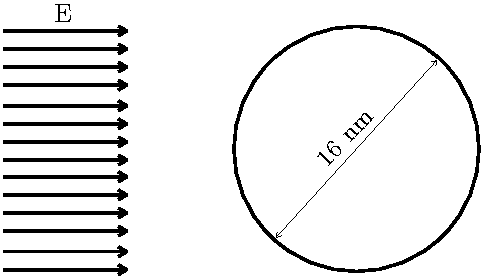
\includegraphics[width=0.55\textwidth]{sphere_field_8nm.pdf} 
    \caption{Spherical nanoparticle in a constant electric field.}
    \label{fig:sph_field}
\end{figure}

\subsection{Grid convergence analysis}\label{sub_sec:grid_conv_iso}

We perform a grid convergence analysis of \pygbe for a silver nanosphere 
of radius $r=8\,nm$ immersed in water, under a z-polarized electric field
of wavelength 380 nm and intensity of $-0.0037 e/(\text{\AA}^2 \, \epsilon_0)$.
For these conditions, the dielectric constant of water is
$1.7972 \, + \, 8.5048^{-09}i$ \cite{HaleQuerry1972} and for silver is
$-3.3877 \, + \, 0.1922i$ \cite{JohnsonChristy1972}. 
Table  \ref{table:quadparams1} shows the Gauss quadrature points used for each 
type of boundary element. We used a threshold parameter to define the near-singular
region of 0.5. This threshold defines the region of near singularity where 
semi-analytical technique is used. If $\sqrt{(2*Area)}/r > \text{threshold}$,
integration is done semi-analytically.
Table \ref{table:treeparams1} lists the parameters for the treecode and solver 
used in this convergence study.

\begin{table}%[h]
    \centering
    \caption{\label{table:quadparams1} Grid-convergence study: Gauss quadrature points; 
    $K$ and $K_{fine}$ are per element; $N_k $ is per element edge (semi-analytical integration). } 
    \begin{tabular}{l l}
    \hline%\toprule
     distant elements: & $K=4$ \\
     near-singular integrals:   & $ K_{fine}=37$ \\
     singular elements:  & $N_k =9$ \\
    \hline%\bottomrule
    \end{tabular}
\end{table}


\begin{table}%[h]
    \centering
    \caption{\label{table:treeparams1} Grid-convergence study: treecode and solver parameters.} 
    \begin{tabular}{l l}
    \hline%\toprule
    treecode order of expansion: & $P=15$\\
    MAC                          & $\theta=0.5$\\
    GMRES tolerance                    & $10^{-5}$\\
    \hline%\bottomrule
    \end{tabular}
\end{table}

Figure \ref{fig:conv_iso_sph} shows the results for the convergence study, with meshes of sizes 512, 2048, 
8192 and 32768 elements. The errors (Table \ref{table:err_iso_sph}) are computed against 
the analytical solution $C_{ext} = 1854.48$ nm$^2$ computed using Equation \eqref{eq:Cext_analytical_lossy}.
The dash line in Figure \ref{fig:conv_iso_sph} corresponds to a $1/N$ slope, and the observed order of 
convergence is $0.98$ which indicates that the meshes are correctly resolving the numerical solution with \pygbe.
The $1/N$ rate of convergence is consistent with the convergence consistent with convergence results in
previous work using \pygbe \cite{CooperBardhanBarba2013}. 

\begin{figure}[h] %  figure placement: here, top, bottom, or page
    \centering
    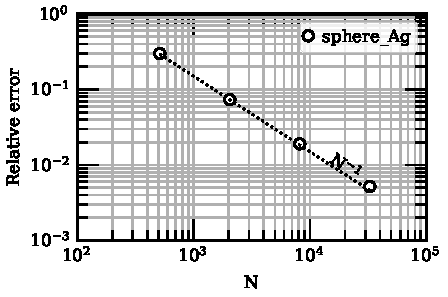
\includegraphics[width=0.65\textwidth]{convergence_sph_Ag_R8_w380.pdf} 
    \caption{Grid-convergence study for the extinction cross-section of a spherical silver
             nanoparticle, computed with \pygbe. Figure, plotting script and auxiliary files 
             available under \textsc{cc-by} \cite{ClementiETal2018c}.}
    \label{fig:conv_iso_sph}
 \end{figure}
 
 
 \begin{table}[h]
     \centering
     \caption{\label{table:err_iso_sph} Percentage error in the grid-convergence cases with an 
     isolated silver nanosphere.} 
     \begin{tabular}{c c}
     \hline%\toprule
     N & \% error \\
     \hline%\midrule
      $512$ & $29.86$ \\
      $2048$ & $7.33$ \\
      $8192$ & $1.9$ \\
      $32768$ & $0.52$ \\
     \hline%\bottomrule
     \end{tabular}
 \end{table}


\subsection{LSPR response of silver nanosphere}\label{sub_sec:lspr_silver_np}

To complement the verification test for the Localized Surface Plasmon Resonance (LSPR) implementation
on \pygbe, we computed the extinction cross section of the isolated silver sphere across multiple 
wavelengths. Figure \ref{fig:verif_sph} shows the results of comparing the simulations with the
analytical solution for a range of wavelengths from $[370-400]$ nm. The values of the dielectric 
for each wavelength were obtained by interpolation of experimental data 
\cite{HaleQuerry1972, JohnsonChristy1972}. To reproduce the interpolation study, we create
a Jupyter notebook and supporting code that can be find as part of the execution files
repro-package \cite{ClementiETal2018b}.
For this verification exercise we use a mesh of $N=32768$, and we relaxed some parameters 
compared to the ones used in the convergence analysis from section \ref{sub_sec:grid_conv_iso} 
that are shown in Tables \ref{table:quadparams2} and \ref{table:treeparams2}. The errors for each 
frequency are below $1\%$, and each runtime decrease by $12\times$.
Figure \ref{fig:verif_sph} exposes a good agreement between the analytical and simulation results, 
showing that \pygbe can accurately represent the mathematical model. Moreover, we can say that 
the level of accuracy is sufficient, given that the experimental uncertainty for the dielectric 
values for silver is in the order of $1\%$ \cite{JohnsonChristy1972}. 

\begin{figure}%[h] %  figure placement: here, top, bottom, or page
    \centering
    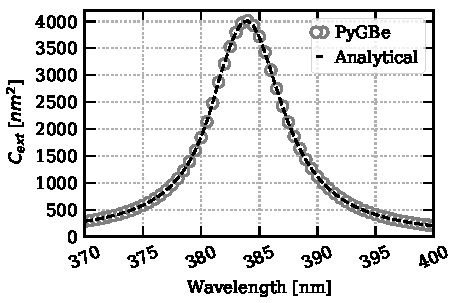
\includegraphics[width=0.65\textwidth]{silver_NP_verification.pdf} 
    \caption{Extinction cross-section as a function of wavelength for an $8$ nm
             silver sphere immersed in water. The peak in the values of 
             extinction cross-section corresponds to the plasmon resonance of the metallic 
             nanoparticle under the incoming electric field. Figure, plotting script and 
             auxiliary files available under \textsc{cc-by} \cite{ClementiETal2018d}.}
    \label{fig:verif_sph}
 \end{figure}

\begin{table}%[h]
    \centering
    \caption{\label{table:quadparams2} Verification: Gauss quadrature points; 
    $K$ and $K_{fine}$ are per element; $N_k $ is per element edge (semi-analytical integration). } 
    \begin{tabular}{l l}
    \hline%\toprule
     distant elements: & $K=4$ \\
     near-singular integrals:   & $ K_{fine}=19$ \\
     singular elements:  & $N_k =9$ \\
    \hline%\bottomrule
    \end{tabular}
\end{table}


\begin{table}%[h]
    \centering
    \caption{\label{table:treeparams2} Verification: treecode and solver parameters.} 
    \begin{tabular}{l l}
    \hline%\toprule
    treecode order of expansion: & $P=6$\\
    MAC                                         & $\theta=0.5$\\
    GMRES tolerance                    & $10^{-3}$\\
    \hline%\bottomrule
    \end{tabular}
\end{table}

% !TEX root = ../thesis-sample.tex

\chapter{LSPR response to Bovine Serum Albumin} \label{chap:lspr_response_bsa}
\graphicspath{{lspr_response_bsa/figs/}}

Localized surface plasmon resonance (LSPR) biosensors detect target molecules
by tracking frequency shifts in the plasmon resonance of metallic nanoparticles
in the presence of analytes \cite{WilletsVandyune2007}. The chapter presents the 
modeling of LSPR biosensors using \pygbe. We compute the extinction cross section 
of a silver nanosphere with bovine serum albumin (BSA) proteins (PDB code: 4FS5,
BSA dimmer) in different locations around it. 


{\color{red}
We might need to add something else here
}

\section{Grid convergence analysis} \label{sec:grid_conv_bsa}
We perform a grid convergence study to ensure that the meshes are correctly
resolving the numerical solutions. We performed the convergence analysis of
the system sketched in in Figure \ref{fig:analyte-sensor}. Given that we 
compute the extinction cross section by integrating over the sphere, we set 
a fixed mesh density for the protein and refined the mesh of the nanosphere 
(512, 2048, 8192, 32768 elements). For the protein, we found that a mesh with
two triangles per $\text{\AA}^2$ was fine enough for the convergence 
analysis, resulting in $N_{prot} = 98116$ elements.
We use the same conditions used in the grid convergence analysis of the 
isolated nanoparticle of section \ref{sub_sec:grid_conv_iso}, presented
in Tables \ref{table:quadparams1} and \ref{table:treeparams1}. The protein 
dielectric constant for a wavelength of 380 nm is $2.7514 + 0.2860i$, this  
value was computed using a functional relationship provided by Phan
 et al.~\cite{PhanETal2013}. The protein was located at a distance of 
 $d=$ 1 nm of the sphere along the z-axis, such that its dipole moment 
 was aligned with the y-axis. We show the errors in Figure  \ref{fig:err_sph-bsa} 
 and table \ref{table:err_sph-bsa} which were computed using the Richardson extrapolated
{\color{red} (see Section, cite section that explains rich extra)} value of 
the extinction cross section $C_{ext}= 1778.73$ nm$^2$.

\begin{figure}%[h] %  figure placement: here, top, bottom, or page
    \centering
    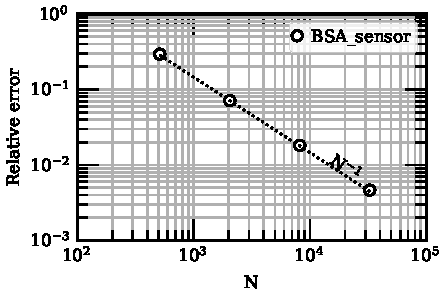
\includegraphics[width=0.65\textwidth]{convergence_bsa_sensor_R8_d1_w380.pdf} 
    \caption{Grid-convergence study of extinction cross-section of a spherical silver
             nanoparticle with a BSA protein at $d=1$ nm. 
             Figure, plotting script and auxiliary files available 
             under \textsc{cc-by} \cite{ClementiETal2018c}.}
    \label{fig:err_sph-bsa}
 \end{figure}

 \begin{table}%[h]
    \centering
    \caption{\label{table:err_sph-bsa} Estimated percentage error of the BSA-sensor 
    system (Fig.~\ref{fig:analyte-sensor}), with respect to the extrapolated value 
    (using Richardson extrapolation).} 
    \begin{tabular}{c c}
    \hline%\toprule
    N & \% error \\
    \hline%\midrule
     $512$ & $29.39$ \\
     $2048$ & $7.13$ \\
     $8192$ & $1.82$ \\
     $32768$ & $0.46$ \\
    \hline%\bottomrule
    \end{tabular}
\end{table}

The observed order of convergence is 0.99, and we can see in Figure
\ref{fig:err_sph-bsa} that the error decays with the number of boundary elements
at a rate of $1/N$, which is consistent with the verifications results showed
in Section \ref{sec:verification}. This shows that the numerical solutions computed
with \pygbe are correctly resolved by the meshes.

\section{Plasmon resonance frequency shifts} \label{sec:shift_bsa}

When a target molecule approaches the metallic nanoparticle, the resonance frequency
of this nanoparticle shifts. In this section, we computed the LSPR response as a
function of the wavelength in the presence of BSA protein. We optimized run times 
without compromising accuracy by using a relaxed set of parameters. For the protein
mesh density we used one element per $\text{\AA}^2$ ($N_{prot} = 45140$) and for the
sphere mesh we used $N_{sensor} = 32768$ elements. These calculations used the same
parameters from Tables \ref{table:quadparams2} and \ref{table:treeparams2}, which 
resulted in a percentage error below $1\%$, with respect to the Richardson-extrapolated
value. The run time for one frequency when two proteins are present, is approximately 
$15$ min using a NVIDIA Tesla K40c GPU.



\begin{center}
    \begin{figure} %  figure placement: here, top, bottom, or page
       \centering
       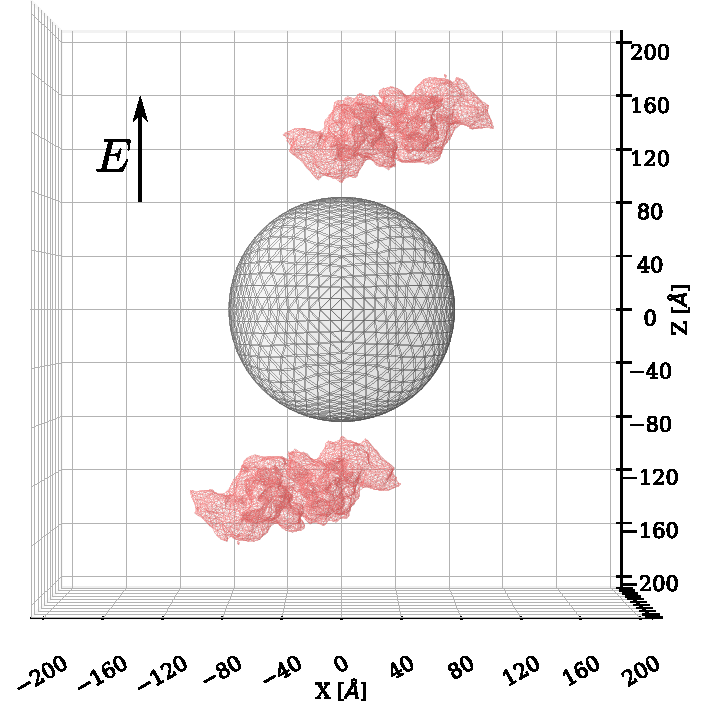
\includegraphics[width=0.65\textwidth]{2prot_1nm_z_R8nm.pdf} 
       \caption{Sensor protein display: BSA located at $\pm 1$ nm of the 
                nanoparticle in the $z$-direction. Figure, plotting script and auxiliary 
                files available under \textsc{cc-by} \cite{ClementiETal2018e}.}
       \label{fig:display_z}
    \end{figure}
    \end{center}

Figure \ref{fig:display_z} shows a visualization of the meshes setup for these 
calculations, with two BSA proteins located at $d=1$ nm away from the spherical 
silver nanoparticle, along the $z$ axis. The position of the BSA molecule at $+z$ 
axis was the same used for the convergence analysis in section \ref{sec:grid_conv_bsa},
while the protein located in the $-z$ position is a 180$^\circ$ solid rotation 
about the $y$ axis, of the BSA in $+z$.  Figure \ref{fig:2pz_response} shows the results
of the calculations between 382 and 387 nm every $0.25$ nm, near the peak seen in Figure
\ref{fig:verif_sph}. In Figure \ref{fig:2pz_response} we have the variation of the 
extinction cross section with respect to wavelength for the isolated nanoparticle 
($d=\infty$) and with BSA proteins located at $d=1$ nm apart from the nanosphere. The
result shows a redshift ($0.5$ nm) in the resonance frequency due to the presence of 
the BSA analytes.

\begin{figure} %[h] %  figure placement: here, top, bottom, or page
    \centering
    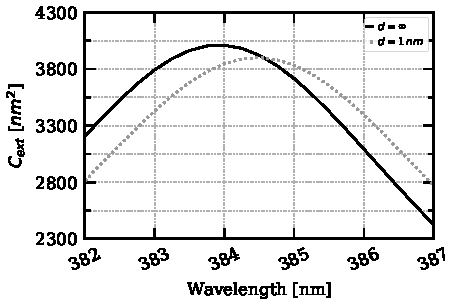
\includegraphics[width=0.65\textwidth]{2pz_R8nm.pdf} 
    \caption{Extinction cross-section as a function of wavelength for an $8$ nm
             silver sphere immersed in water with two BSA proteins placed 
             $\pm 1$ nm away from the surface in the $z$-direction, and at
             infinity (no protein).}
    \label{fig:2pz_response}
 \end{figure}

Figure \ref{fig:2pz_response} shows a redshift of the plasmon resonance frequency 
peak in the presence of two BSA proteins located at 1 nm along the $z$ axis. Experimental 
observations in the work of Tang, et al.~\cite{TangETal2010} revealed a redshift when 
BSA proteins in a solution are added to silver nanoparticles of approximately $17$ nm 
in diameter. They also observed a decrement of the peak amplitude, similarly to the 
effects we see with our model. Moreover, recent experiments \cite{PuETal2018} report 
resonance frequency between $380$ and $400$ nm for a silver nanosphere in the presence
of BSA proteins (check reference and its supplementary material), which is consistent with 
our results. Other experiments \cite{RaphaelETal2013} also report redshifts in the presence
of different proteins. The boundary element method approach that we implemented using 
electrostatic approximation is thus able to capture the characteristics of LSPR biosensors
based on resonance-frequency shift. 

We also study the effect of the location of the proteins, we performed the same 
calculations but now placing the BSA analytes along the $x$ and $y$ axis at $\pm 1$ nm,
as shown in Figure \ref{fig:display_xy}. We obtain these configurations by performing
a 90$^\circ$ solid rotation of the $z$-configuration (Figure \ref{fig:display_z})
along the $x$- and $y$-axis, respectively. Figure \ref{fig:2pxy_response} shows the 
results for each configuration.

 \begin{figure}
    \centering
    \subfloat{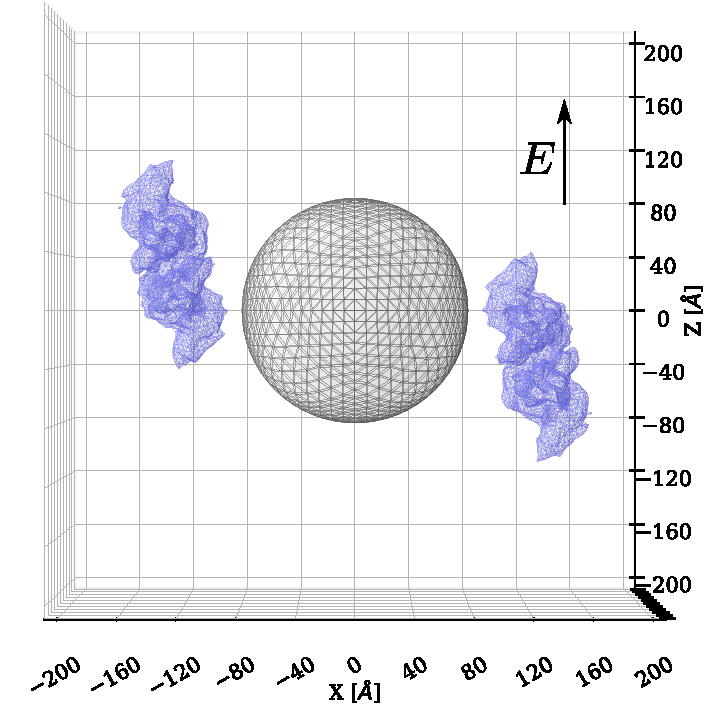
\includegraphics[width=0.65\textwidth]{2prot_1nm_x_R8nm.pdf}} \\
    \subfloat{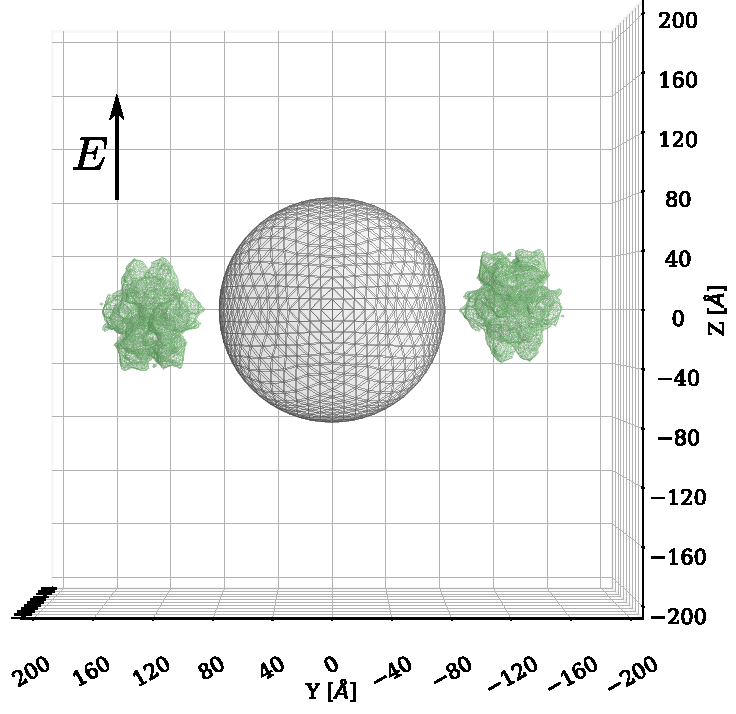
\includegraphics[width=0.65\textwidth]{2prot_1nm_y_R8nm.pdf}} 
     \caption{Sensor protein display: BSA located at $\pm 1$ nm of the nanoparticle in the
            $x$-direction (top) and $y$-direction (bottom). Figure, plotting script and 
            auxiliary files available under \textsc{cc-by} \cite{ClementiETal2018e}.}
     \label{fig:display_xy}
 \end{figure}

 \begin{figure}%[t] %  figure placement: here, top, bottom, or page
    \centering
    \subfloat{\includegraphics[width=0.65\textwidth]{{2px_R8nm}.pdf}}\\
    \subfloat{\includegraphics[width=0.65\textwidth]{{2py_R8nm}.pdf}} 
    \caption{Extinction cross-section as a function of wavelength for an $8$-nm
             silver sphere immersed in water with two BSA proteins placed at
             $\pm 1 $ nm away from the surface in the $x$-direction (top) and
             $y$-direction (bottom), and at infinity (no protein).}
    \label{fig:2pxy_response}
 \end{figure}

Figure \ref{fig:display_xy} shows the configuration where the proteins are placed at a 
distance in the $x$ (top) or $y$ (bottom) direction. For these configurations and with 
the electric field aligned with the $z$ axis, the LSPR response is negligible. The 
frequency shifts in Figure \ref{fig:2pxy_response} are smaller than the wavelength 
resolution ($<0.25$ nm). This finding is consistent with the free electrons oscillating
along the $z$ axis under a $z$-polarized electric field, and not in the $x$ and $y$ 
directions {\color{red} ADD REFERENCE TO FIG OF OSCILLATING ELECTRONS - LSPR}. The 
proteins have a marked effect when placed in the $z$ direction, where they can interfere 
with the oscillation of the free electrons. 

\section{Sensitivity study} \label{sec:sensitivity}

On LSPR biosensors we refer to sensitivity to the relationship between the size of the 
resonance frequency shift and the number of analytes bound to the sensor (through the 
ligand). Experiments show that the distance between the protein and the nanoparticle 
affects the sensitivity of the sensor, to the point that targets placed 15 nm away 
from the surface are hardly detectable \cite{HaesETal2004}. This is a critical issue
considering that most common ligands, like antibodies, can be larger than 15 nm. In 
Figure \ref{fig:dist_response} we can see how the resonance peak varies with the distance 
at which the  analytes are located ($+z$ and $-z$). When $d=2$ nm we have a shift of 
$0.25$ nm while when the analytes are at $d=0.5$ nm the shift is $0.75$ nm. The parameters
used in these simulations remain the same as the ones used for the cases in Figures 
\ref{fig:2pz_response} and \ref{fig:2pxy_response}.

\begin{figure}%[h] %  figure placement: here, top, bottom, or page
   \centering
   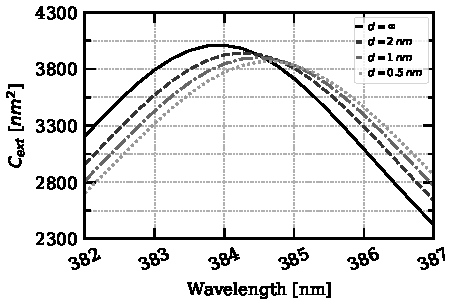
\includegraphics[width=0.65\textwidth]{2pz_lspr_response.pdf} 
   \caption{Extinction cross-section as a function of wavelength for an $8$-nm
            silver sphere immersed in water with two BSA proteins placed at
            $2$, $1$, and $0.5$ nm away from the surface in the 
            $z$-direction, and at infinity (no protein). The test case with
            $d=0.5$nm is close to the limit where quantum tunneling might happen. 
            Such effects are not captured by our classical model.}
   \label{fig:dist_response}
\end{figure}

As expected, Figure \ref{fig:dist_response} shows how the shift decreases as the BSA 
proteins move away from the nanoparticle, to the point that we only see a shift of 
$0.25$ nm when the analyte is $2$ nm away. This results shows the potential of \pygbe 
and the electrostatic approach to study biosensors sensitivity with distance. It's 
worth noting that quantum effects (e.g., tunneling) at $d=0.5$ nm are ignored with 
our classical approach. Even if this distance could be close to the quantum regime, 
there is evidence that classical theory is valid at this distance in similar systems
\cite{SavageETal2012, EstebanETal2012}

Even though there is evidence that techniques such as plasmon-enhanced Raman 
scattering are capable of detecting to the single-molecule limit 
\cite{ZhangZhangETal2013}, as far as we know there is no evidence of a purely
LSPR approach that can sense such low concentrations of proteins. Our 
computational results can unveil potential improvements that would enhance 
the sensitivity of LSPR biosensors, for example by using smaller ligands. 

There are not other LSPR simulations where the molecular details of the analyte 
are considered, that we are aware of. However, similar calculations can be 
performed with other open source softwares like BEM++ \cite{SmigajETal2015} and 
MATLAB toolbox MNPBEM \cite{HohenesterTrugler2012}. BEM++ also models the system
as a set of boundary integral equations, discretized in flat triangular panels, 
and it uses a Galerkin approach and algorithmic acceleration via hierarchical 
matrices. MNPBEM is another alternative software designed to simulate scattering
of metallic nanoparticles, which its BEM implementation is similar to \pygbe 
(centroid collocation with flat triangles) but with different acceleration scheme.
This MATLAB toolbox, similarly to BEM++, also relies on hierarchical matrices 
rather than a treecode, resulting in higher memory usage compared to our code, 
making it harder to simulate large analytes in detail. 
Commercial finite-element or finite-difference solvers can also be used for this
type of application, for example COMSOL. However, these volumetric approaches 
struggle to correctly impose the zero boundary condition at infinity, which is
exactly met for BEM.  


%Next big section should be on Reduced order model for protein in LSPR applications
%Here we will put all the results of: pqr effect, ellipsoids effects, dielectric effect.
% !TEX root = ../thesis_main.tex

\chapter{Reduced order model for protein representation}

In the literature there are several reports that use Bovine Serum Albumin as an analyte
to simulate the behavior of a bioconjugate sensor. However, they use a simplified model
of the protein. For example, a layer of protein-water solution \cite{PhanETal2013}, 
or just a protein dielectric layer \cite{NghiemETal2012}, others model the
protein as a triangular prism \cite{DanHu2014}, or even a small sphere with a 
constant dielectric \cite{SantiagoCordobaETal2011, UngerETal2009}. Phan and 
coworkers \cite{PhanETal2013} present a Lorentz-Drude model for the complex 
dielectric of the BSA which we use in our work, while most of the literature 
use a constant dielectric with no losses to represent the BSA 
(refractive index of $n= 1.9$ \cite{NghiemETal2012}, $n= 1.45$ \cite{SantiagoCordobaETal2011}) or
other proteins used as analytes ($n=1.58$ polystrene \cite{UngerETal2009}, $n=1.57$ 
streptavidin \cite{ShenETal2013}). 

Research shows that the shape of both monomer and dimmer of 
BSA are prolate ellipsoids \cite{MoserETal1966, SquireETal1968, WrightETal1975}. However,
this is information, to the best of our knwoledge, hasn't been used to model the 
protein in computational approaches. Our BSA model, based on its crystal 
structure, can be consider as a good reference of the actual shape of the protein. We 
explore the effects of using reduced-order models, like ellipsoids, by comparing 
the results with the full model, and study the consequences of these 
simplifications. We study the effect of the shape and volume of the protein
(see section CITE SECT) as well as the presence of charges in it. 

To the best of our knowledge, there is no model in the literature that counts 
for the charges inside the protein. We study the effect on the LSPR response 
in the presence and omission of charges and how this varies depending on the 
intensity of the incoming electric field (see section CITE SECT).\\  

% Surface Phonon Polaritons resonance: Replication and Validation studies
% !TEX root = ../thesis_main.tex

\chapter{Replication and Validation studies}

HERE WE SHOULD HAVE A PARAGRAPH THAT GOES OVER WHAT WE DID IN THESE 2 CASES
% !TEX root = ../thesis_main.tex

\section{Replicating Rockstuhl et al 2005} \label{chap:rep_rockstuhl}
\graphicspath{{replication_validation/figs/}}

When looking for results to attempt the validation of \pygbe we found the study of Rockstuhl et al. 2005 \cite{rockstuhl2005}. 
Even though their work consist on simulations and therefore does not qualify for a validation study, we decided to 
attempt the replication of one of their results. 

Rockstuhl and coworkers, in their paper "Analysis of the phonon-polariton response of silicon carbide microparticles 
and nanoparticles by use of the boundary element method", study the phonon-polariton response of silicon carbide (SiC)
nanoparticles using boundary element method. They use a two dimensional model developed previously on their group \cite{rockstuhl2003}
to analyze 6H-SiC multiple "cylindrical particles" (third dimension tends to infinity). The results presented on Figure 14 of their paper  
present the scattering cross-section of a SiC rectangular cylinder for different aspect ratios, and the case with $a = 672$ nm and $b = 328$ nm
was a perfect candidate given that these dimensions comply with our quasistatic approach.

In the work of Rockstuhl et al., they compute scattering cross section while with \pygbe we compute the extinction cross-section 
(absorption plus scattering). In the quasistatic regime absorption dominates over scattering, therefore these results are not directly
comparable. However, when having materials which show narrow and sharp peaks on their spectra, the wavelength at which the peaks occur 
in the scattering and extinction spectra, are nearly the same. For example, in the work of Wiley et al. \cite{wiley-etal-2006}
we see that for a silver nanocube, the wavelength at which the main peaks occur for extinction and scattering, are nearly the same. Due to the properties 
of silicon carbide, its spectra presents sharper and narrower peaks than silver, which leads to closely aligned extinction and scattering peaks.


\textbf{Differences in method and input data}

\begin{itemize}

\item {The main difference between the simulations in Rockstuhl and the ones performed with \pygbe is that the original results where obtained 
using a 2D boundary element method that solves full Maxwell equations, while we solve a 3D problem with the quasistatic limit approximation.}

\item{ Rockstuhl et al. work did not have a section with details on their simulations such as discretization of the geometries or parameters 
involved in their simulations. We chose parameters for our solver based on our previous experiences, and for the discretization of our 
geometries we performed a grid-independence study to ensure that we are minimizing discretization errors. It is worth noting that Rockstuhl
et al. geometries consist in two dimensions (infinite third dimension), while we perform the computations using a full 3D representation of the geometry.} 

\item {Regarding the complex dielectric constant, the study we aim to replicate uses 6h-SiC and their data comes from a source that we were not able
to replicate. As a replacement, we are using experimental data of 4H-SiC provided to us by the authors of Ellis et al. \cite{ellis2016} via 
private communications.}

\end{itemize}

\subsection{Grid independence study} \label{ssec:grid_indep_rock}

The equations that we solve in this problem are the same as the ones we solved in chapter \ref{chap:iso_silver_np} where we show grid convergence for the case of 
a silver sphere. In the work of Rockstuhl et al. \cite{rockstuhl2005} the geometries are cubes and prisms, and due to the nature of the geometries 
and their sharp edges, it was hard to find a case where we could see proper convergence using richardson extrapolation. Since we have show convergence for this type of physics
for the case of the sphere and given the difficulty of the sharp edges, we decided to settle with a grid-independence study. We performed the grid-independence study
on a similar setup to the case ib Fig. 18 of Rockstuhl et al. \cite{rockstuhl2005}, a cube of side $L=535$ nm surrounded by air, under a constant electric field aligned with the 
z-axis. Figure \ref{fig:cube535} shows the grid-independence study where we use a mesh with 15,552 triangles and a 19,200 triangles 
(from 9.05 $\times$ 10$^{-5}$ to 1.11 $\times$ 10$^{-4}$ triangles per $\text{\AA}$ squared) and the computed results are indistinguishable from each other.
We want to remark that the spectrum presented in Figure \ref{fig:cube535} has an extra peak compared to the one presented in Fig. 18 of Rockstuhl et al. \cite{rockstuhl2005}. We attribute
this extra peak to the three-dimensional nature of the geometry used in our model and the sharp edges, the latter effect also being mentioned by the Rockstuhl et al.
In the following sections we will present the replication study of one of the results on Figure 14 of Rockstuhl et al. and we will the effects of the 3D model as well as the sharpness of the edges. 

\begin{figure}
    \centering
    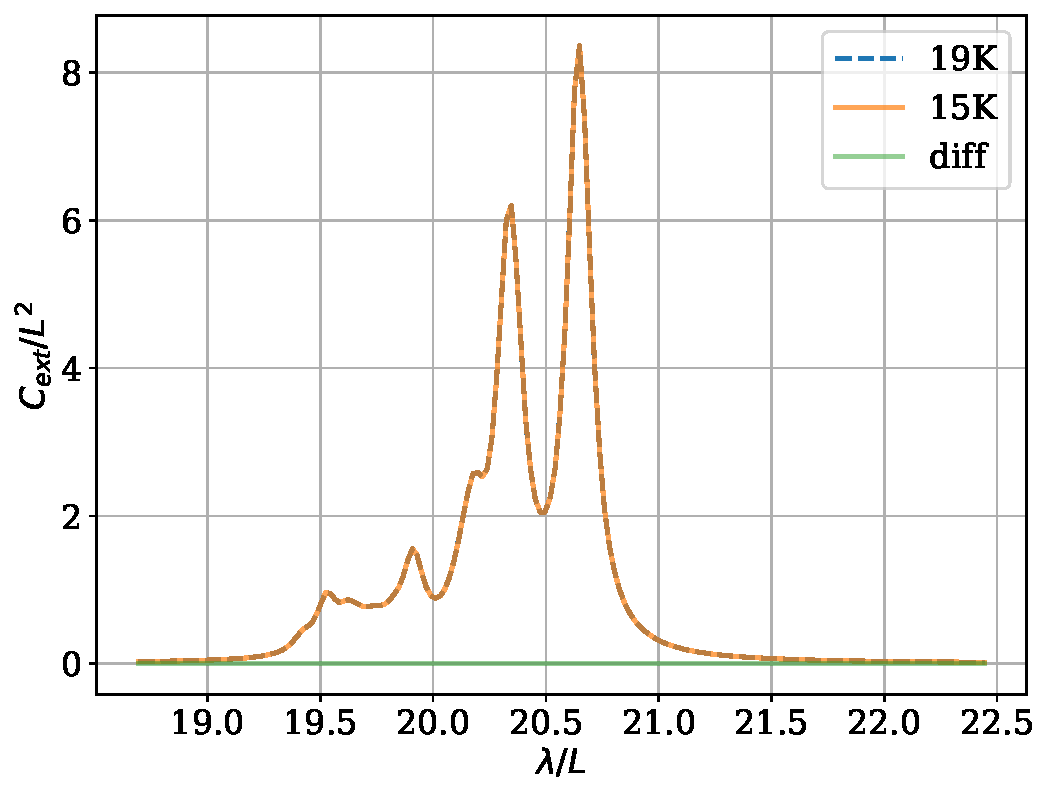
\includegraphics[width=0.75\textwidth]{cubeL535nm_15Kvs19K.pdf} 
    \caption{Grid-independence study for a SiC cube of side $L=535$ nm submerged in air under a constant 
    electric field in the $z$-direction. The curves represent the extinction cross-section divided by $L^2$ 
    as a function of wavelength divided by $L$, for mesh sizes 19K = 19,200 triangles and 15K = 15,552 triangles. 
    The label "diff" refers to the difference between the results of the two meshes.}
    \label{fig:cube535}
 \end{figure}

 \subsection{Replication of Figure 14 (case a1) of Rockstuhl et al., 2005}

 We chose to replicate the case "a1" ($a=672$ nm and $b=328$ nm) from the Figure 14 from Rockstuhl et al., 
 this case has dimensions that are within the quasistatic limit used in \pygbe. Rockstuhl and coworkers show the normalized
 scattering cross-section of a SiC rectangular cylinder, and they perform simulations for the setups showed in the Figure
 \ref{fig:rectangle_sketch}. In Figure \ref{fig:rectangle_sketch} (A) the electric field is parallel to the long side of the geometry, which 
 corresponds to the configuration of Figure 14 (right) of Rockstuhl et al. where the wave vector (illumination) goes along the short side of the geometry. 
Similarly, we see that in Figure \ref{fig:rectangle_sketch} (B) the electric field is parallel to the short side of the geometry, which 
corresponds to the configuration of Figure 14 (left) of Rockstuhl et al. where the wave vector (illumination) goes along the long side of the geometry
For the mesh of the rectangular prisms we used densities like the ones used in the grid-independence study (section \ref{ssec:grid_indep_rock}) or finer. We needed to elongate
the third dimension to the point that it represented "infinity". Figure \ref{fig:ext_y_14} shows the results of extending the third dimension ($y$ axis) to 
$y=1344$ nm ($2\times a$) and $y=2688$ nm ($4\times a$). We can see that when $y$ takes the longer value, the intensity of some peaks decreases, due to their association to 
the y-component. We have not explored larger values of $y$ because are limited by the quasistatic limit.
 \begin{figure}
    \centering
    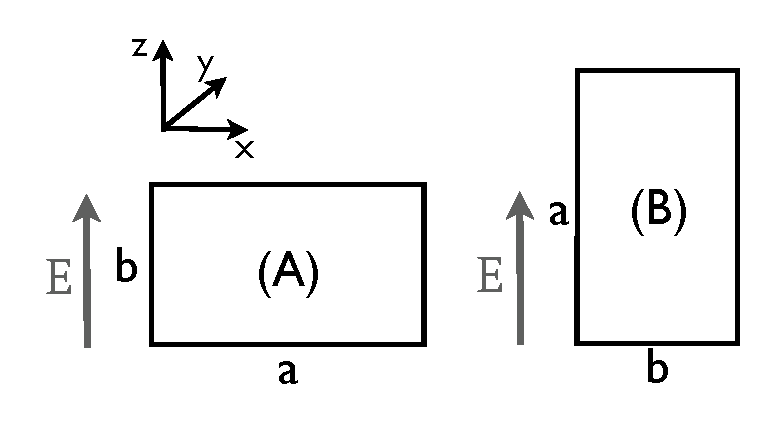
\includegraphics[width=0.45\textwidth]{rockstuhl_rectangles.pdf} 
    \caption{Configurations for the simulations corresponding to Fig. 14 of Rockstuhl et al., 2005.}
    \label{fig:rectangle_sketch}
\end{figure}

\begin{figure}
    \centering
    \subfloat{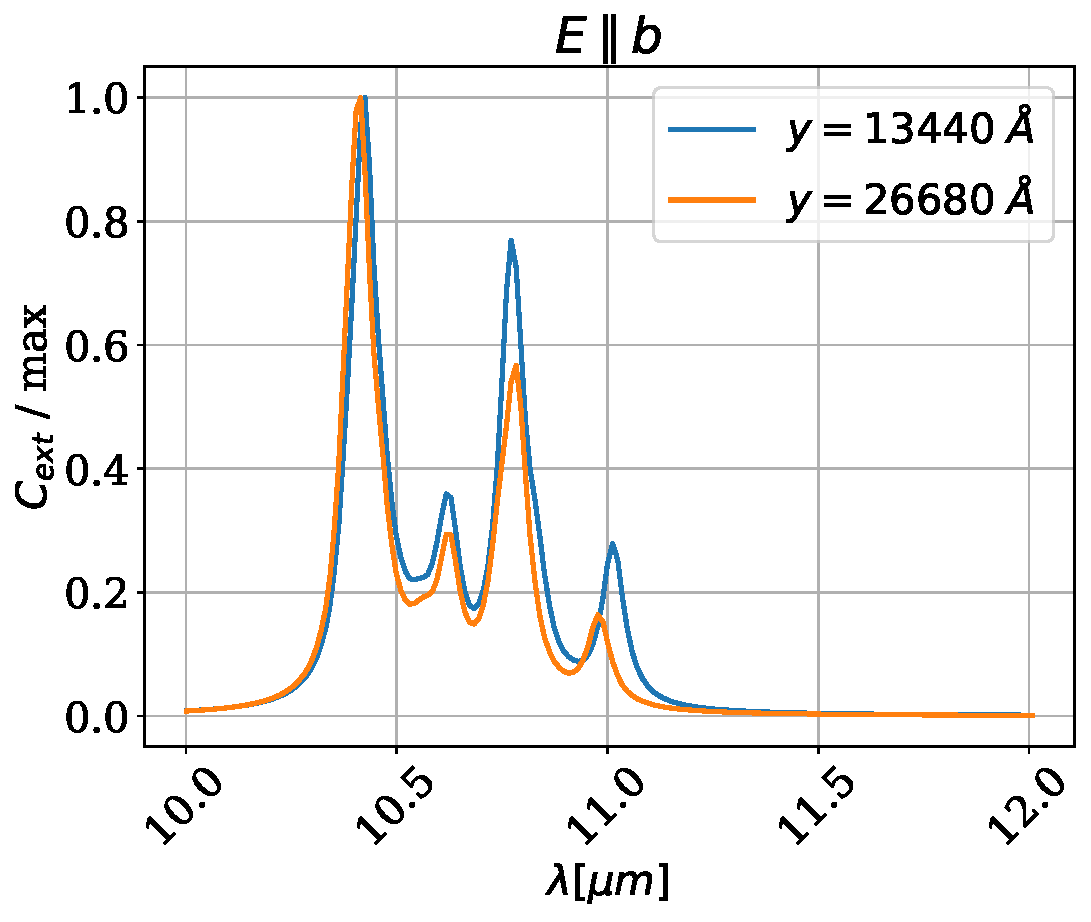
\includegraphics[width=0.48\textwidth]{ext_y_14a.pdf}}
    \subfloat{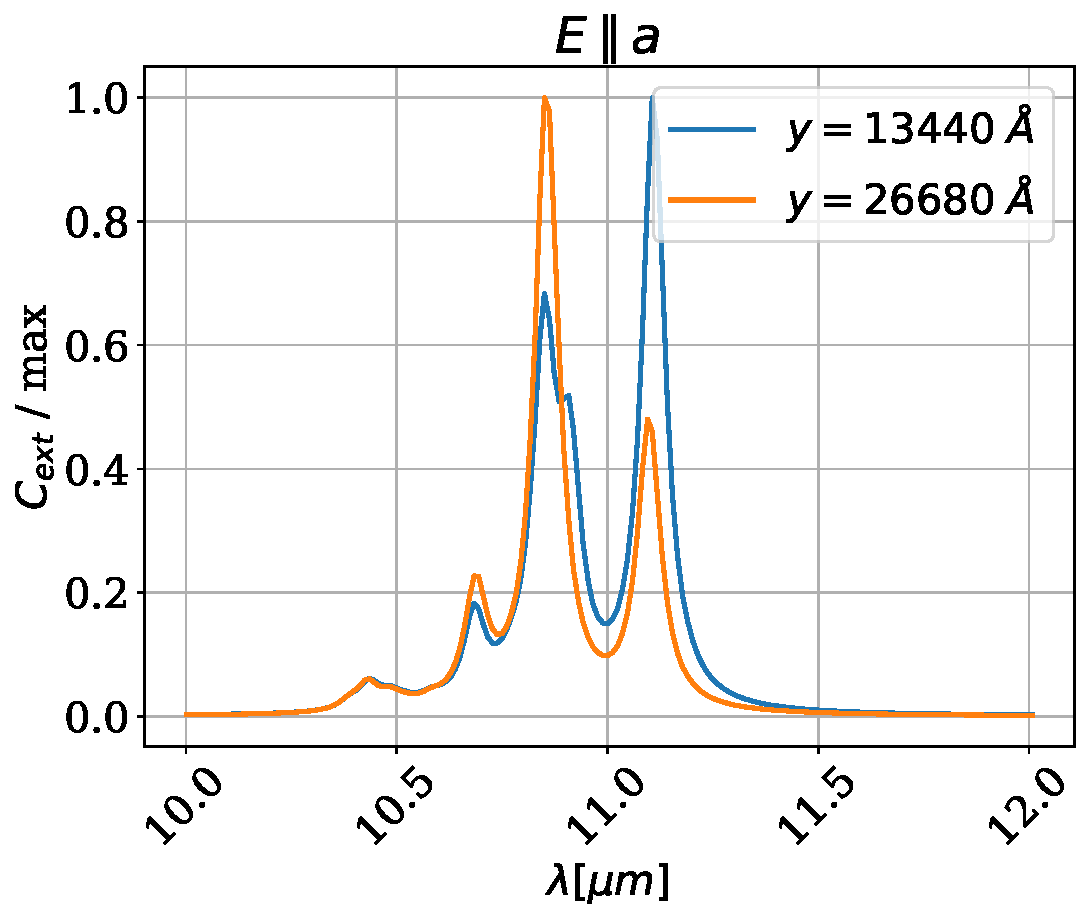
\includegraphics[width=0.48\textwidth]{ext_y_14b.pdf}} 
    \caption{Effect of the elongation of the third dimension ($y$) on the 
        extinction cross-section of a rectangular prism of SiC of dimensions $a=672$ nm 
        and $b=328$ nm, submerged in air and under a constant electric field 
        parallel to the $z$-axis. The left plot corresponds to a configuration such that the electric 
        field is parallel to $b$ (configuration (A) on Figure \ref{fig:rectangle_sketch}), while the 
        right plot corresponds to a configuration such that the electric field is 
        parallel to $a$ (configuration (B) on Figure \ref{fig:rectangle_sketch}.}
    \label{fig:ext_y_14}   
 \end{figure}

For the simulations of Figure \ref{fig:ext_y_14} we generated the meshes using an open source software Trimesh (\url{https://github.com/mikedh/trimesh}), 
but we realized that the mesher did not produce a uniform mesh and that it was not possible to obtained one with the functions available. To solve this problem 
we created a uniform mesh with our own Python script. We wanted to study the effect of using a uniform mesh and the roundness of the edges, the latter being mentioned by 
Rockstuhl et al. as a cause of the appearance of extra peaks. To generate the roundness of the geometries we relied on Trimesh (we give as input the uniform mesh generated 
with our Python script), however, we did not have control of the roundness as a function of the geometry dimensions or arc of curvature, so we used the default settings of
the software. Figure \ref{fig:tri_reg_round_14} shows the results of the effect of mesh uniformity and roundness of the edges of the geometry. We can see that in the for 
both orientation of the geometry ($E\parallel b$ and $E\parallel a$) the second peak located at $\approx$ 10.6 $\mu$m is much diminished in the green curve. These effects 
can be attributed to the roundness of the edges, what is consistent with the results of Rockstuhl et al. Once we have found the "best" meshed geometry (uniform mesh plus 
round edges) that we can construct, we can compare our results (green curve \ref{fig:tri_reg_round_14}) with the ones in Rockstuhl et al. Figure 14. We present the replication 
results in Figure \ref{fig:rep_14}, and we can see that the main resonance peaks in Figure 14 of Rockstuhl et al. are closely matched. We still have a third peak in our 
results, but we attribute this to the effects introduced by using a 3D geometry. We obtained the data from Rockstuhl's curves by using the WebPlotDigitizer
(\url{https://apps.automeris.io/wpd/}).
 

 \begin{figure}
    \centering
    \subfloat{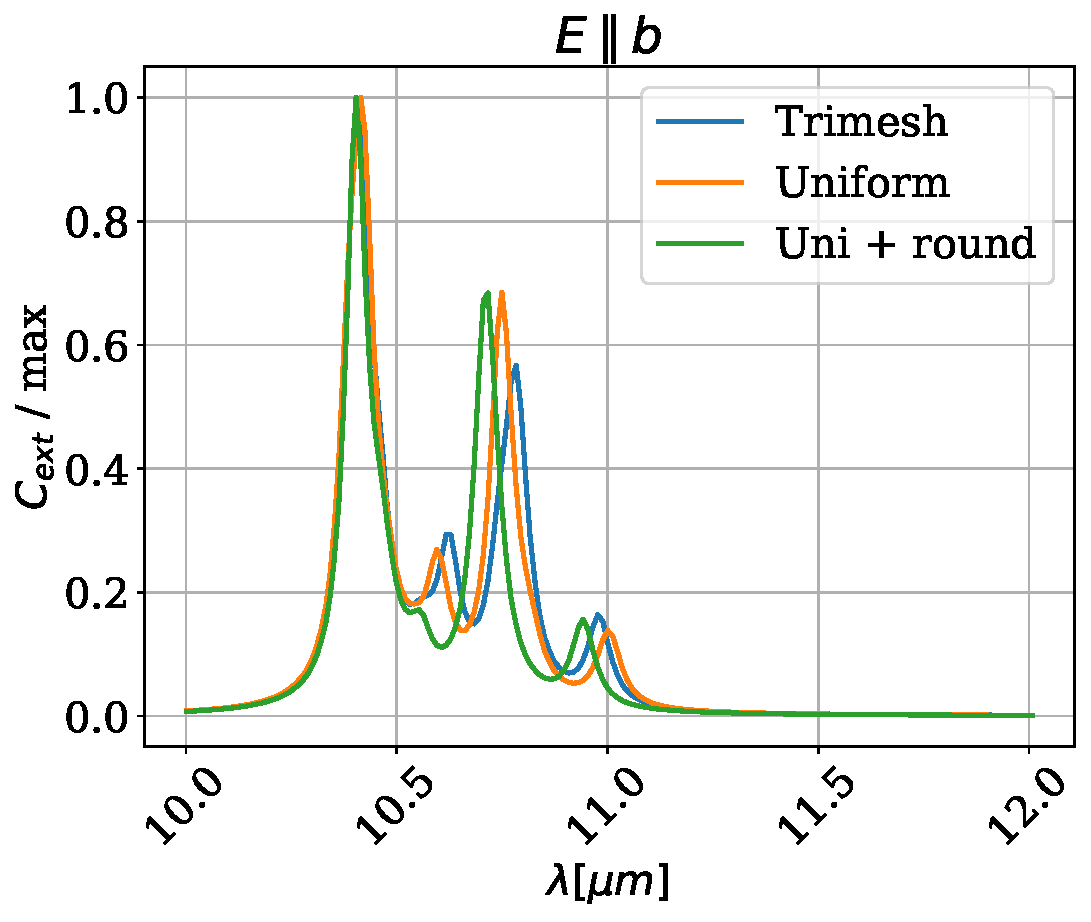
\includegraphics[width=0.48\textwidth]{tri_reg_round_14a.pdf}}
    \subfloat{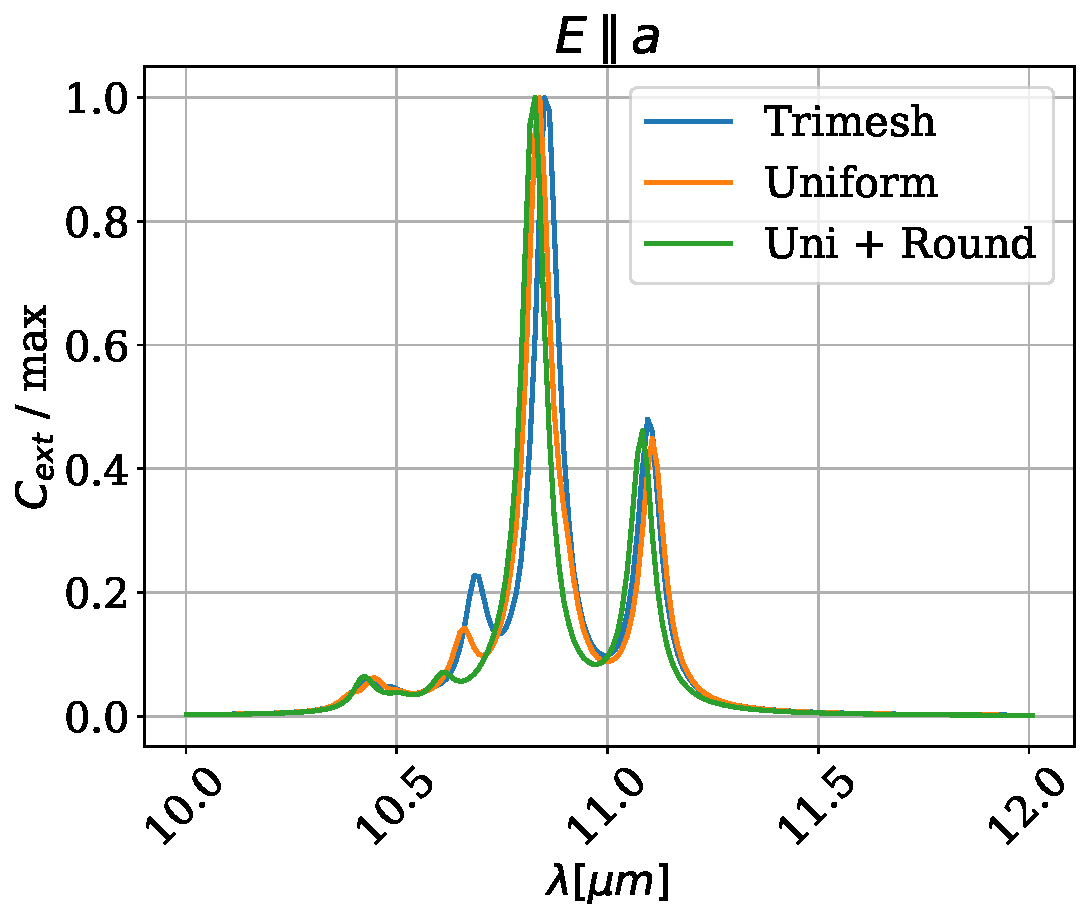
\includegraphics[width=0.48\textwidth]{tri_reg_round_14b.pdf}}
    \caption{Effect of uniformity of the mesh and roundness of the edges on the 
    extinction cross-section of a rectangular prism of SiC of dimensions $a=672$ nm, 
    $b=328$ nm and $y=2688$ nm, submerged in air and under a constant electric field 
    parallel to the $z$-axis. The labels are: \textbf{Trimesh}, for a non-uniform mesh generated using Trimesh; 
    \textbf{Uniform}, for a uniform mesh generated using Python scripts; and 
    \textbf{Uni + round}, for a uniform mesh generated using Python scripts with round 
    edges obtained using Trimesh.}
    \label{fig:tri_reg_round_14}
 \end{figure}

 \begin{figure}
    \centering
    \subfloat{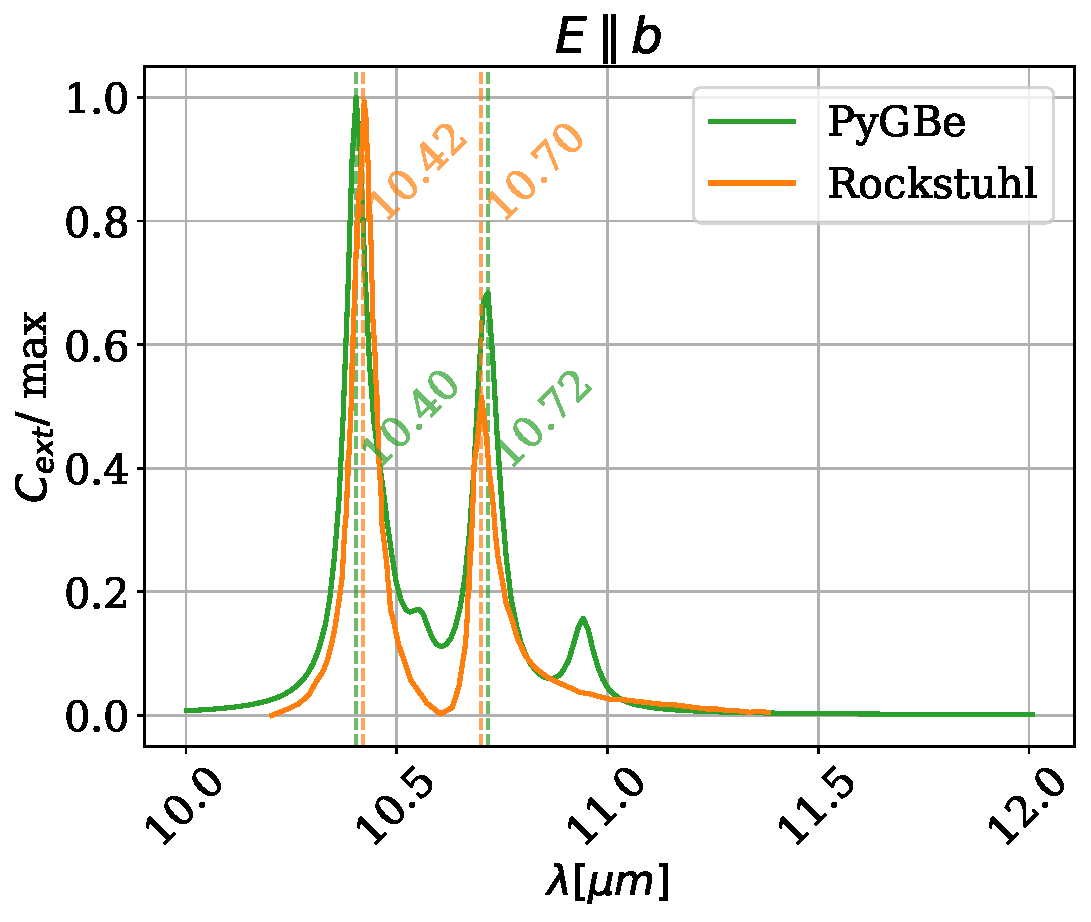
\includegraphics[width=0.48\textwidth]{replication_14a.pdf}}
    \subfloat{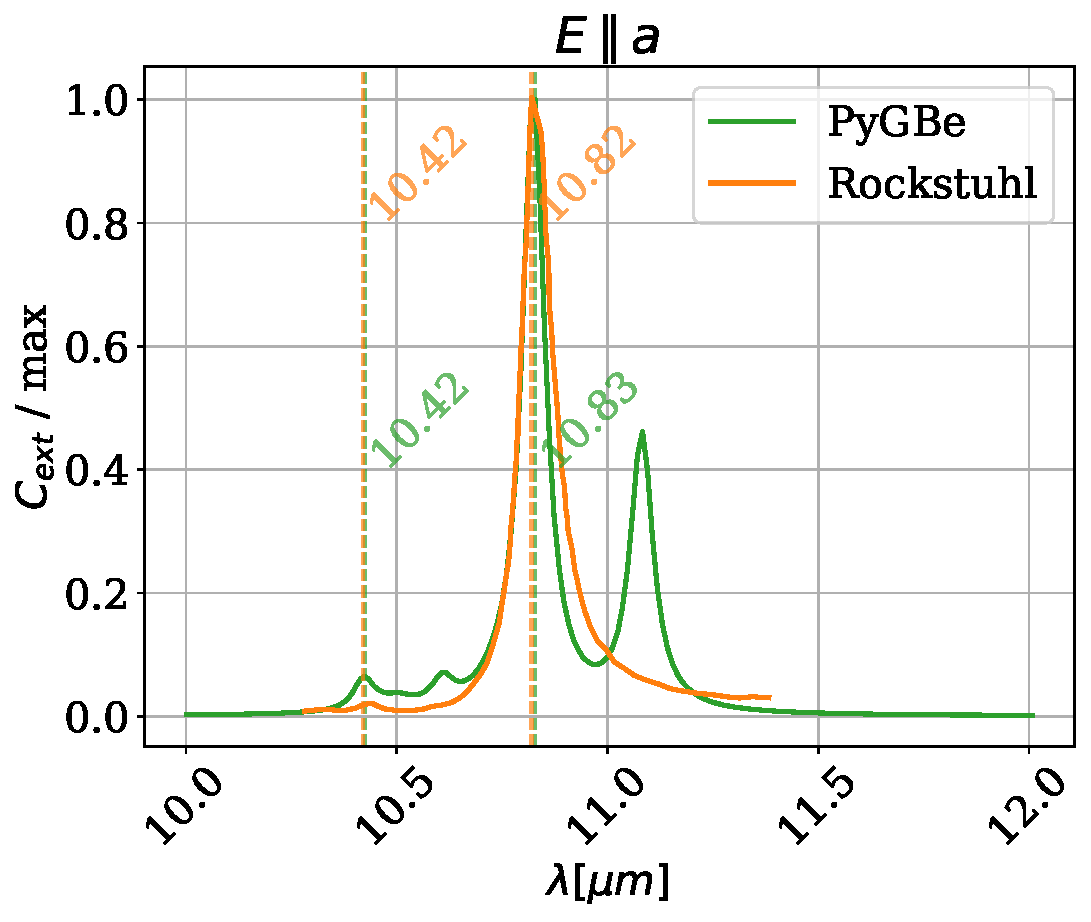
\includegraphics[width=0.48\textwidth]{replication_14b.pdf}} 
    \caption{Replication of the results in Figure 14 of Rockstuhl et al., 2005. Extinction cross-section of a
    rectangular prism of SiC of dimensions $a=672$ nm, $b=328$ nm and $y=2688$ nm, submerged
    in air and under a constant electric field parallel to the $z$-axis (green line). 
    The digitized curve from Rockstuhl et al.\ corresponds to scattering (orange line).}
    \label{fig:rep_14}
 \end{figure}
% !TEX root = ../thesis_main.tex

\section{Validation of \pygbe and Replication of Ellis et al. 2016  et al 2005} \label{sec:rep_val_ellis}
\graphicspath{{replication_validation/figs/}}

The work of Ellis et al. "Aspect-ratio driven evolution of high-order resonant modes and near-field distributions in
localized surface phonon polariton nanostructures." \cite{ellis2016} has both computational and experimental results, that makes 
it a perfect candidate to perform a validation as well as a replication study. Ellis and coworkers study the excitation of 
multipolar localized surface polaritons (SPhP), by computing and measuring the polarized reflectance on 4H-SiC pillars of
fixed width ($W = 400$ nm), fixed height ($H=950$ nm) and varied length ($L=400-4800$ nm). To reduce coupling, these pillars are 
pattern on a square grid with $P = L + 500$ nm. In their experiments (simulations), they measure (compute) the polarized reflectance
where the incident polarization is oriented parallel or perpendicular to the length ($L$) of the pillars. We started by replicating a 
computational result shown in Figure S4 of their supplementary material. Figure S4 of the 
supplementary material shows simulation results for the resonance spectral position of the lower frequency mode when the angle of 
incidence is $22$ degrees and the polarization is parallel to the length of the pillars. They present results for separations of $500$ nm 
(red curve) and $5000$ (black curve), the latter a good candidate for replication with \pygbe because a larger gap diminishes 
the coupling (not included in our model). The setup in our computations consists of a single pillar with no substrate.
Secondly, we aimed to replicate the results of Figure 2a of the main paper, 
corresponding to reflectance measurements across the wave number for pillars of aspect ratio $AR=4$, angle of incidence 22 degrees, 
and incoming parallel polarization. For this case the authors also reported experimental results and we used them for the 
validation of our solver. For all the simulations involved in the replication and validation studies we use experimental values of the 
complex dielectric data for 4H-SIC provided by the authors of Ellis et al. via private communication. 

\textbf{Differences in method and input data}

\begin{itemize}

\item {The simulations of Ellis et al. compute the solution of Maxwell's equations using the RF package
of the finite element solver in the commercial software COMSOL. Their setup consists of one pillar over a 
substrate, with periodic boundary conditions to emulate the array of pillars used in their experiments. In our 
solver we use the boundary element method in the quasistatic approximation, which is suitable since the wavelengths
involved are in the range $10000-12500$ nm, and are considerably larger than the pillar's dimensions. We compute 
the extinction cross section, where the resonance expresses as peaks instead of dips as in the reflection plots of 
Ellis et al. The intensity of the peaks is not comparable, however, we are looking to match the wave number at which
they happen.}

\item {The simulations of Ellis et al. rely on a volumetric model and use a volumetric mesh. In our 
solver, the geometries are represented as a triangular surface meshes. For the validation and replication of Figure 2a of 
their paper, where the pillars have an aspect ratio of $AR=4$, we use a non-uniform triangular mesh ($N=4398$) that 
was provided by the authors of Ellis et al. However, for the replication of the Figure S4 of the supplementary material, 
we were missing the remaining meshes for the other aspect ratios. To overcome this, we generated the meshes with our Python 
script, and we determined the density to be used by comparing simulations for the case of aspect ratio $AR=4$ of our mesh and 
the one provided by Ellis and coworkers. Using approximately double the number of elements ($N=8564$) than the original mesh 
and rounding the edges using Trimesh, the relative errors for the extinction cross-section were, on average, smaller than 
$3\%$, and the variations on the wave number of the peak position was smaller than $1$cm$^-1$. After this analysis we 
concluded in a density of $\approx \; 1.7 \times10^{-5}$ triangles per $\text{\AA}$ squared, which we used to create the meshes
for the remaining aspect ratio geometries.}

\item {In Ellis et al. they perform simulations for different angles of incidence of the illuminating vector. To achieve this 
using \pygbe we rotated the geometry, since the direction of the illuminating vector in our solver is fixed.}
\end{itemize}

\subsection{Replication of Figure S4 of supplementary material of Ellis et al. 2016}

To replicate Figure S4 of the supplementary material we identify the lower-frequency mode for every different 
aspect ratio in our computations. For the values of aspect ratio ($AR$) from 1 to 7, we computed the extinction cross section 
$C_{ext}$ across wave numbers in the range of $800-1000$ cm$^{-1}$, and we identified the lower-frequency mode 
($E^{\parallel}_{100}$ for Ellis et al.) that was not a longitudinal mode. The longitudinal modes are the ones associated with 
the height of the pillar and they appear only when we have an angle of incidence that is off-normal. 
Figure \ref{fig:AR_22_vs_norm} shows the results of the extinction cross-section of a SiC pillar for different values of 
length ($L=400$-$2800$ nm), for normal and 22-degrees angle of incidence (see Figure \ref{fig:ellis_ang_inc}). We performed 
the simulations for the long-edge orientation, meaning that the electric field is aligned with the length of the pillar when having a normal 
incidence. From each result of Figure \ref{fig:AR_22_vs_norm}, we selected the lowest non-longitudinal mode and extracted the corresponding wavelength
(see Table \ref{tab:ar_peaks}) to replicate Figure S4 of the supplementary material of Ellis et al. Figure \ref{fig:rep_FS4_ellis} shows the
results from Ellis et al. (obtained using the WebPlotDigitizer) and the results obtained using \pygbe. Table \ref{tab:err_AR} contains the 
percentage error and we can see that is below 2$\%$ for all the cases.

\begin{figure}
    \centering
    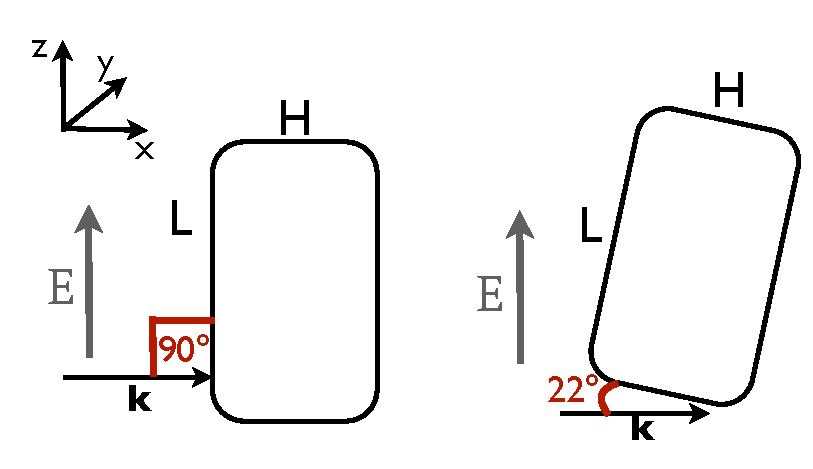
\includegraphics[width=0.45\textwidth]{ellis_ang_inc.pdf} 
    \caption{Diagram showing the angles of incidence in our simulation setups to comply with the configuration in the case from Ellis et al.}
    \label{fig:ellis_ang_inc}
\end{figure}

\begin{figure}
    \centering
    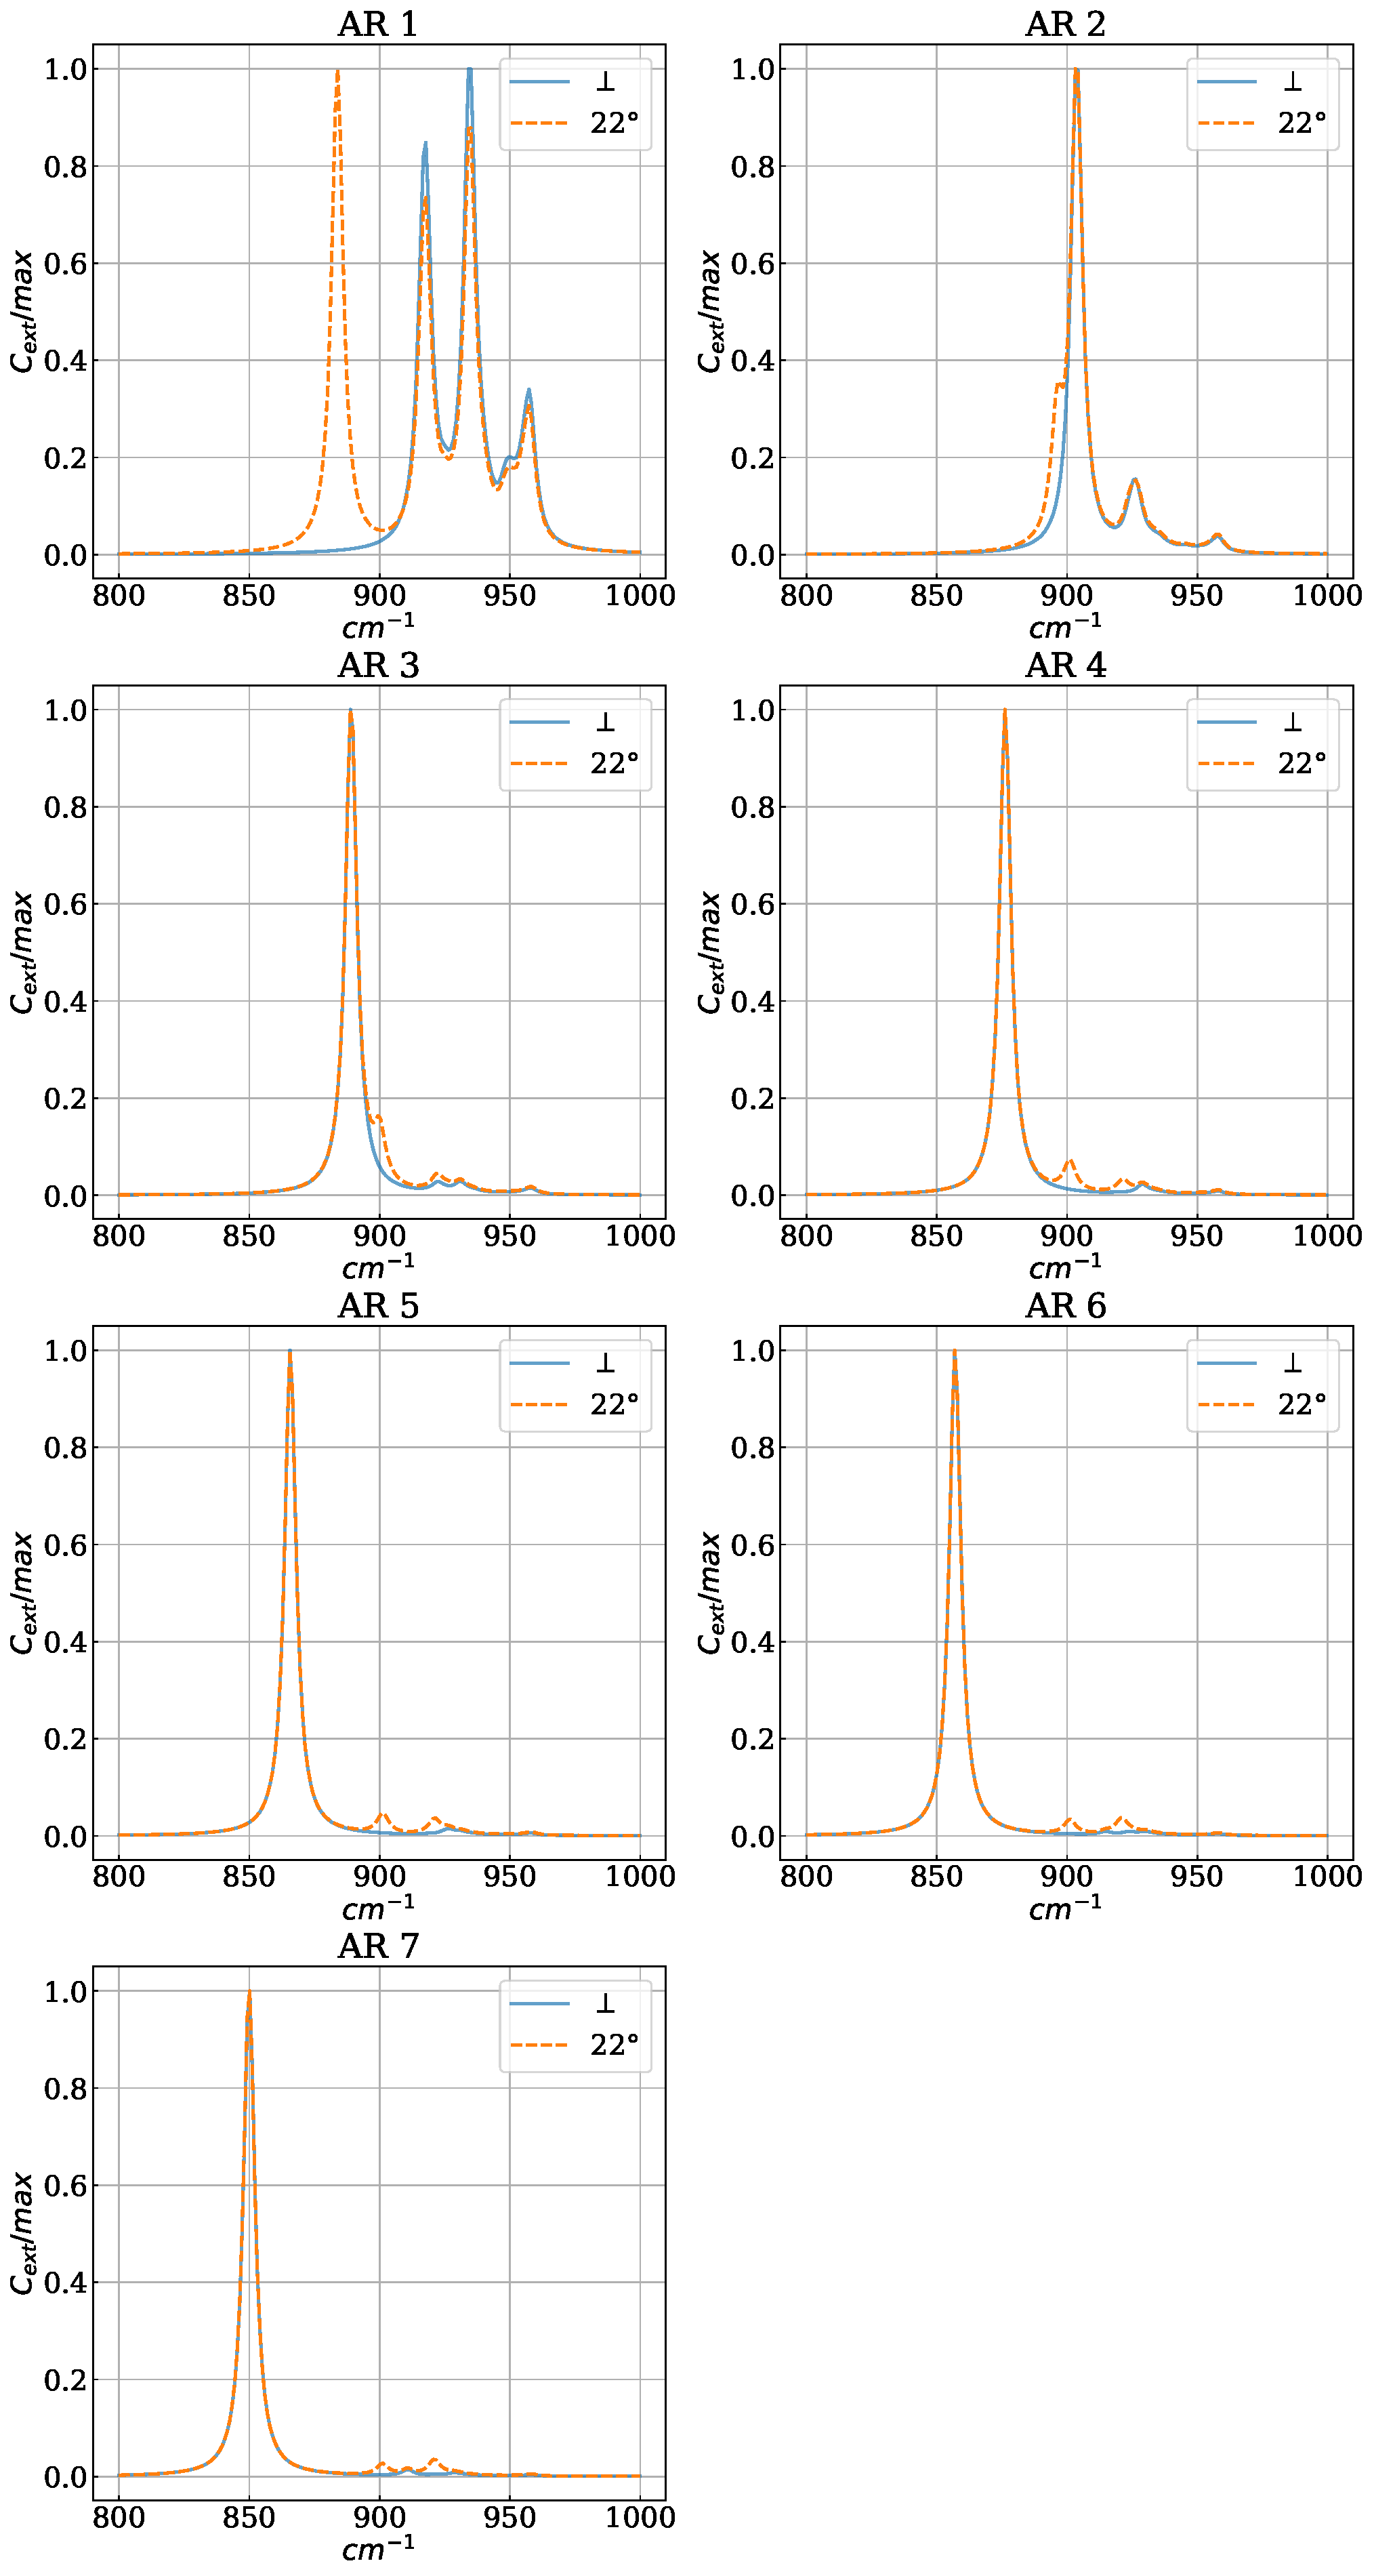
\includegraphics[width=0.72\textwidth]{AR_22_vs_norm.pdf} 
    \caption{Extinction cross-section across wave numbers for SiC pillars of varying aspect ratios,  
             ($H=950$ nm, $W=400$ nm, $L=400$--$2800$ nm, $AR=1$--$7$), with both normal incidence and a 
             22-degree incidence.}
    \label{fig:AR_22_vs_norm}
\end{figure}

\begin{table}
    \centering
      \caption{Wavelength at which peaks happen for different aspect ratios, for runs where the electric
      field is parallel to the length ($L$) of the pillar. We have normal incidence and 22-degree incidence.
      The wavelengths in bold correspond to the lowest mode that is not a longitudinal one.}
      \label{tab:ar_peaks}
      \begin{tabular}{c c c c c c c c}
        \textbf{AR} \\
        \hline
        \multirow{2}{*}{1} & $\perp$ & \textbf{917.73} & 934.092 & 949.604 & 957.325 \\ % <-- Combining 2 rows with arbitrary with (*) and content 12
        & 22$^{\circ}$ & 883.926 & \textbf{917.73} & 935.052 & 949.604 & 957.325 \\ % <-- Content of first column omitted.
        \hline
        \multirow{2}{*}{2} & $\perp$ & \textbf{903.233} & 926.395 & 944.762 & 958.242 \\ % <-- Combining 2 rows with arbitrary with (*) and content 12
        & 22$^{\circ}$ & 896.517 & \textbf{903.233} & 926.395 & 944.762 & 958.242 \\ % <-- Content of first column omitted.
        \hline
        \multirow{2}{*}{3} & $\perp$ & \textbf{888.793} & 922.552 & 931.223 & 948.613 & 958.242 \\ % <-- Combining 2 rows with arbitrary with (*) and content 12
        & 22$^{\circ}$ & \textbf{888.793} & 899.418 & 922.552 & 931.223 & 958.242 \\ % <-- Content of first column omitted.
        \hline
        \multirow{2}{*}{4} & $\perp$ & \textbf{876.186} & 929.32 & 946.639 & 958.242 \\ % <-- Combining 2 rows with arbitrary with (*) and content 12
        & 22$^{\circ}$ & \textbf{876.186} & 901.281 & 921.618 & 929.32 & 945.745 & 958.242 \\ % <-- Content of first column omitted.
        \hline
        \multirow{2}{*}{5} & $\perp$ & \textbf{865.576} & 926.395 & 945.745 & 958.242 \\ % <-- Combining 2 rows with arbitrary with (*) and content 12
        & 22$^{\circ}$ & \textbf{865.576} & 901.281 & 921.618 & 958.242 \\ % <-- Content of first column omitted.
        \hline
        \multirow{2}{*}{6} & $\perp$ &  \textbf{856.904} & 914.793 & 923.489 & 929.32 & 946.639 & 958.242\\ % <-- Combining 2 rows with arbitrary with (*) and content 12
        & 22$^{\circ}$ & \textbf{856.904} & 901.281 & 920.6 & 958.242\\ % <-- Content of first column omitted.
        \hline
        \multirow{2}{*}{7} & $\perp$ &  \textbf{850.134} & 910.963 & 921.618 & 928.372 & 946.639 & 958.242 \\ % <-- Combining 2 rows with arbitrary with (*) and content 12
        & 22$^{\circ}$ & \textbf{850.134} & 901.281 & 910.963 & 920.6 & 958.242\\ % <-- Content of first column omitted.
        \hline
      \end{tabular}
\end{table}

\begin{figure}
    \centering
    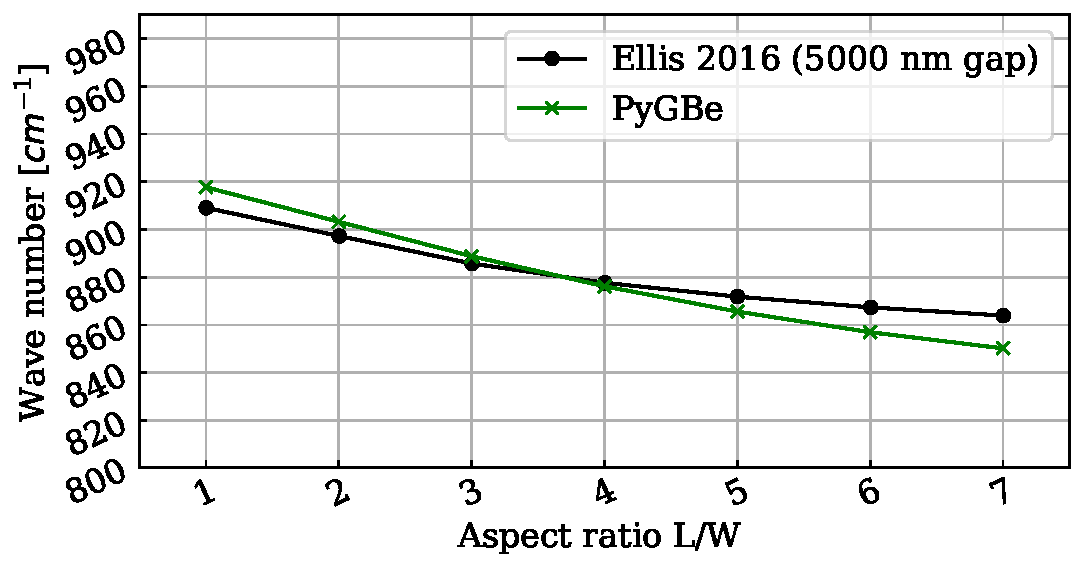
\includegraphics[width=0.85\textwidth]{AR_rep_FS4_Ellis2016.pdf} 
    \caption{Replication of figure S4 in the supplementary materials of Ellis et al., 2016. Wave
    number at which the $E^{\parallel}_{100}$ mode happens for different aspect ratios.}
    \label{fig:rep_FS4_ellis}
 \end{figure}
 
 \begin{table}
    \centering
    \caption{Percentage error for different aspect ratios.} 
    \label{tab:err_AR}
    \begin{tabular}{c c}
    \hline%\toprule
    AR & \% error \\
    \hline%\midrule
     $1$ & $0.95$ \\
     $2$ & $0.67$ \\
     $3$ & $0.35$ \\
     $4$ & $0.16$ \\
     $5$ & $0.72$ \\
     $6$ & $1.20$ \\
     $7$ & $1.59$ \\
    \hline%\bottomrule
    \end{tabular}
\end{table}

\subsection{Validation of \pygbe against experimental results in Fig. 2a of Ellis et al., and replications
of the corresponding computations}\label{ssec:validation}

The geometry used in the results of Figure 2a of Ellis et al. correspond to the case of aspect ratio $AR=4$. For this case,
we have the mesh provided by the authors. Since our computation for the mode $E^{\parallel}_{100}$ compares well with 
their results (percentage error of $0.16\%$), we chose this particular result from Ellis et al. to validate our simulations 
with their experimental results (red curve on their paper), as well as to replicate its corresponding computations (green 
curve on their paper). Figure 2a of Ellis et al. shows experimental and computational results of the reflectance of SiC pillar 
arrays with a gap of 500 nm, where the angle of incidence is 22$^\circ$ off-normal and the incoming polarization is parallel 
to the length of the pillar. Using \pygbe, we computed the extinction cross section of an isolated SiC pillar of aspect ratio
$AR=4$ with no substrate, submerged in air and under a constant electric field in the $z$-direction. The geometry was rotated to match
the angle of incidence of 22$^\circ$ used by Ellis et al. (see Figure \ref{fig:ellis_ang_inc}). Figure \ref{fig:pygbe_vs_exp_2a} 
shows the comparison of our simulations and the experimental results of Ellis et al. We can observe a noticeable difference in between 
the wave numbers at which the peaks occur. This difference may be attributed to the fact that in their experimental setup the 
separation between the pillars is $500$ nm, which implies there are coupling effects that are not considered in our simulations.

\begin{figure}
    \centering
    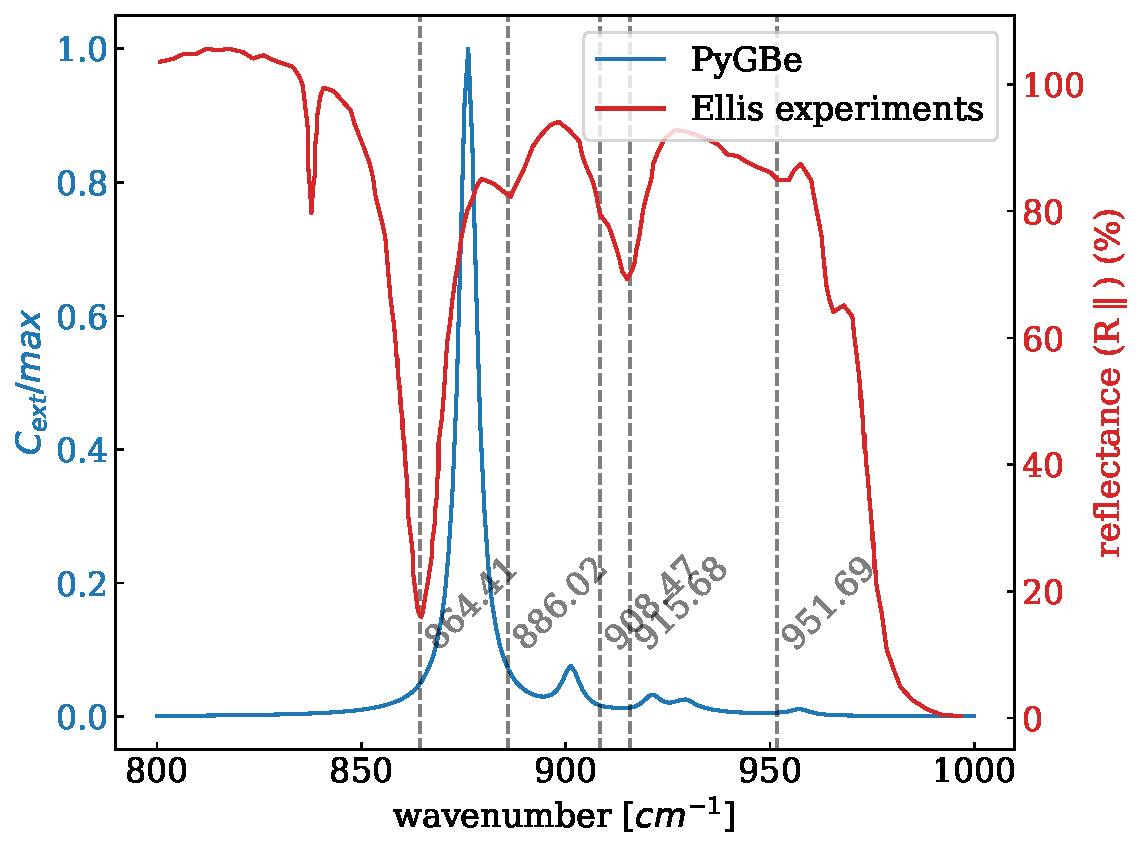
\includegraphics[width=0.85\textwidth]{pygbe_vs_exp_fig2a_Ellis.pdf} 
    \caption{\pygbe vs.\ the experiments presented in Figure 2a of Ellis et al., 2016 (we obtained the data 
    digitizing by hand from their figure using WebPlotDigitizer).}
    \label{fig:pygbe_vs_exp_2a}
 \end{figure}

\textbf{First-order correction.} 

Since our simulations are performed on an isolated prism and do not take into account the coupling effects 
in an array of prisms, we cannot strictly match the conditions to validate our solver. However, from Figure S4 in the supplementary material of 
Ellis et al., we know that this coupling effects affect the $E^{\parallel}_{100}$ mode by a shift of 12.17 cm$^{-1}$. Then, as a 
\textbf{first-order correction}, we can subtract this amount from our computations to account for the coupling effects. Figure \ref{fig:val_2a}, 
shows the results after applying the correction. It is worth mentioning that the peaks at 837 cm$^{-1}$) and (964 cm$^{-1}$) on the results of Ellis et al., 
are associated with the zone-folded LO (longitudinal) phonons of 4H-SiC, an effect they say to be beyond the scope of their analysis \cite{ellis2016}. Their 
analysis concentrates on the peaks that occur between 864 cm$^{-1}$ and 961 cm$^{-1}$. 
Figure \ref{fig:rep_2a} shows the comparison between Ellis et al. simulation's results on Figure 2a of their paper (green curve), and our computations
after applying the first-order correction.

\begin{figure}
    \centering
    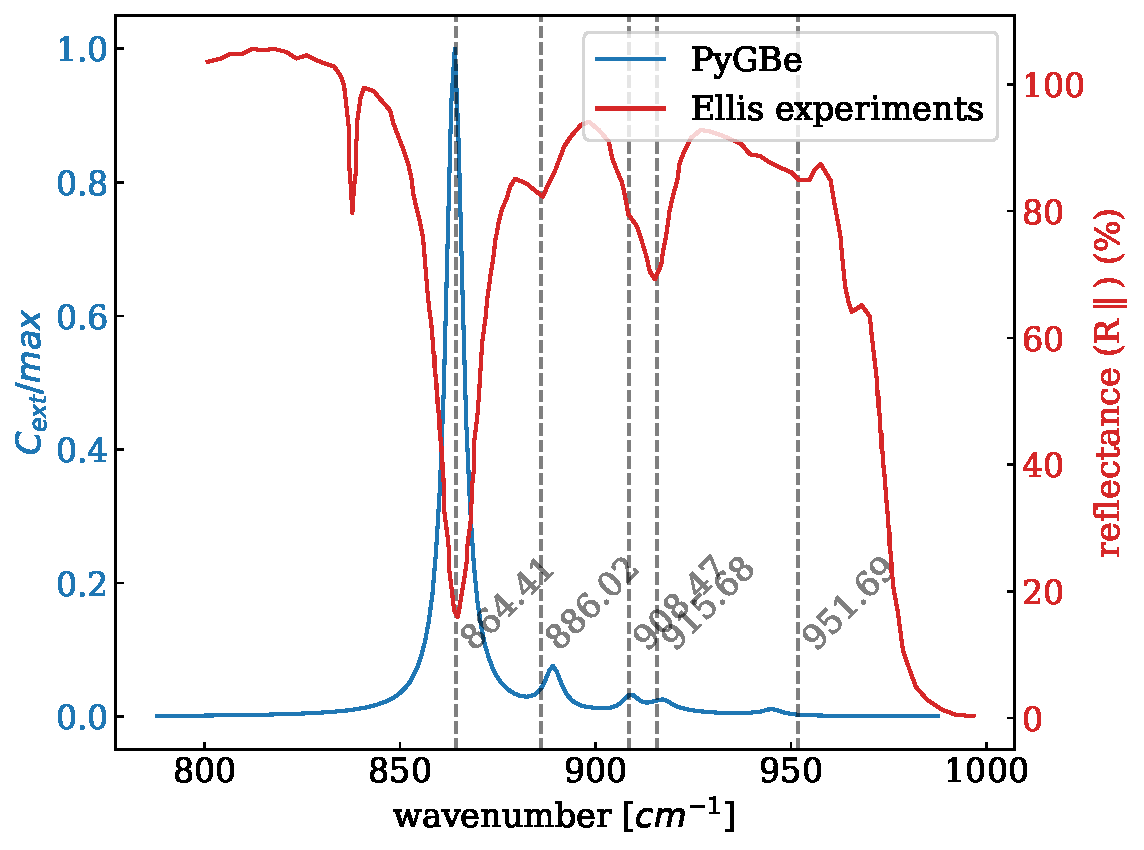
\includegraphics[width=0.85\textwidth]{validation_FOA_fig2a_Ellis.pdf} 
    \caption{Validation against experiments in Figure 2a of Ellis, et al., 2016, using the first-order correction, as explained in the text.}
    \label{fig:val_2a}
 \end{figure}

\begin{figure}
    \centering
    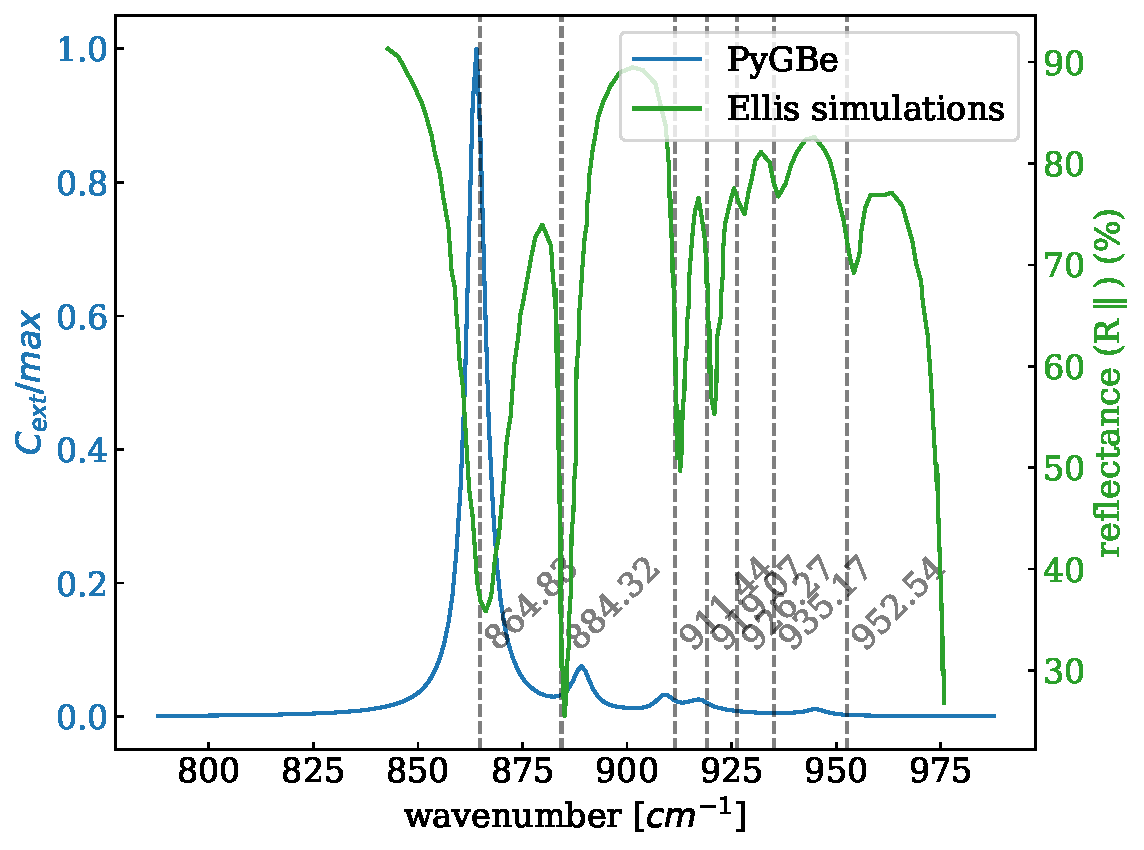
\includegraphics[width=0.85\textwidth]{replication_FOA_fig2a_Ellis.pdf} 
    \caption{Replication of the simulations in Figure 2a of Ellis et al., 2016, using the first-order correction, as explained in the text.}
    \label{fig:rep_2a}
 \end{figure}


In this section, we attempted to replicate two results from Ellis et al. \cite{ellis2016} where they study the effect of aspect ratio on the 
excitation of high-order modes in localized surface phonon-polariton nanostructures. Figure \ref{fig:rep_FS4_ellis} shows the results for
the replication of the black curve of Figure S4 of their supplementary material, where the relative errors between our computations and 
theirs is always smaller than 2$\%$. This replication study gave us the confidence to approach the replication of Figure 2a of Ellis et al., 
given that in that case they use a geometry with aspect ratio $AR=4$ presented the smallest error (see Table \ref{tab:err_AR}). Since 
Figure 2a of Ellis et al. shows results of experiments and simulations with the commercial software COMSOL, we not only pursued replication 
but we also sought the validation of \pygbe using these experimental results. The quantity plotted in the original figures is reflectance as a 
function of wavenumber, while we compute the extinction cross section. Since the quantity of interest is the wavenumber at which the resonance 
peaks/dips happen, the results are comparable. 

Figure \ref{fig:pygbe_vs_exp_2a} shows the results of our simulations using \pygbe on an isolated pillar, compared with the experimental results
of Ellis et al.\ on an array of pillars. The results with \pygbe do not account for the effect of coupling among the pillars, which explains the  
discrepancy on the wavenumbers at which the peaks occur. It is worth mentioning that we did not count with the original data behind the plots of 
Ellis et al. therefore, we digitize the curves using the WebPlotDigitizer(\url{https://apps.automeris.io/wpd/}). Based on the results reported 
on Figure S4 of Ellis et al.\ for the $AR=4$ case, we proposed a first order correction that subtract the shift on the wave number due to
coupling is 12.17 cm$^{-1}$ (difference between black and red curves for $AR=4$ on figure S4 of the supplementary materials). Figure \ref{fig:val_2a}
and Figure \ref{fig:rep_2a} show the comparison of our corrected results with their experiments and simulations, respectively. We observe a good match 
of the wavenumber for the lower (and stronger) mode, as well as a good match for the third and fourth peaks. The wave number of the second peak, related 
to a longitudinal excitation (mode $L_{000}$ in Ellis et al.), presents a discrepancy that we believe is related to the fact that our 
pillar does not have a substrate underneath. The remaining (fifth) peak, also presents a discrepancy, but in this case we could not identify the reason.
We did not analyze the peaks out of the range 864--961 cm$^{-1}$, since Ellis et al.\ describe these peaks to be associated with 
zone-folded LO (longitudinal) phonons of 4H-SiC, and outside the scope of their study.
After considering all these details, we can say that we have validated our solver \pygbe against the experimental results of 
Figure 2a, as well as replicated their computational results.

\section{Reproducibility and data management} \label{sec:repro_val}
 
All the results of this chapter have been accepted for publication in the journal 
Philosophical Transactions A \cite{ClementiBarba2020} and can be reproduced or replicated. \pygbe is openly developed and 
shared under the BSD3-clause license via its repository at \url{https://github.com/pygbe/pygbe}.

All results of this chapter were obtained on a lab workstation, built from parts. Hardware specifications are as follows:

\begin{itemize}
  \item CPU: Intel Core i7-5930K Haswell-E 6-Core 3.5GHz LGA 2011-v3
  \item RAM: G.SKILL Ripjaws 4 series 32GB (4 x 8GB)
  \item GPU: Nvidia Tesla K40c (with 12 GB memory)
\end{itemize}

Readers can reproduce all the figures in this chapter using the repro-packs shared in Zenodo. They include 
data and scripts needed to run the calculations reported in this chapter, the manually digitized data from the figures
in the source articles for our replication cases, as well as Jupyter notebooks with all the plotting code:

\begin{itemize}

\item[$\triangleright$] The problem datasets for replication of Rockstuhl et al., 2005, are in the manuscript repository, but also archived in Zenodo  at \href{https://doi.org/10.5281/zenodo.3962534}{10.5281/zenodo.3962534}  \cite{ClementiBarba2020-Zen_a}.

\item[$\triangleright$] Execution files for all runs are archived in Zenodo at \href{https://doi.org/10.5281/zenodo.3962576}{10.5281/zenodo.3962576} \cite{ClementiBarba2020-Zen_b}.

\item[$\triangleright$] The problem datasets for validation and replication of results from Ellis et al., 2016 are archived in Zenodo at \href{https://doi.org/10.5281/zenodo.3962584}{10.5281/zenodo.3962584}\cite{ClementiBarba2020-Zen_c}.

\item[$\triangleright$] The file sets for reproducing the figures for the replication of results from Rockstuhl et al., 2005 are archived in Zenodo at \href{https://doi.org/10.5281/zenodo.3962791}{10.5281/zenodo.3962791} \cite{ClementiBarba2020-Zen_d}.

\item[$\triangleright$] The file sets for reproducing the figures for the validation and replication of results from Ellis et al., 2017 are archived in Zenodo at \href{https://doi.org/3962797/zenodo.3962797}{10.5281/zenodo.3962797} \cite{ClementiBarba2020-Zen_e}.

\end{itemize}


\bibliographystyle{plain}
\bibliography{thesis_ncc_bib}

% appendices must appear after
%\include{tex/appendix}
\end{document}
